%----------------------------------------------------------------------
% MasterThesis: Ekaterina Tikhoncheva, © 09/2015
%----------------------------------------------------------------------
\documentclass  [
  paper    = a4,
  BCOR     = 10mm,    % binding correction
  twoside,
  fontsize = 12pt,
%  fleqn,
  toc      = bibnumbered,
  toc      = listofnumbered,
  numbers  = noendperiod,
%  headings = normal,
  listof   = leveldown,
  chapterprefix=true  % like in standard class "report"
]                                       {scrbook} %{scrreprt} %{scrbook}
% used pagages
\usepackage     [utf8]                  {inputenc}
\usepackage     [T1]                    {fontenc}
\usepackage     [sc]                    {mathpazo} % Palatino für Mathemodus
%\usepackage                             {exscale} 
\usepackage                             {microtype}
%\usepackage                             {color}
\usepackage                             {xcolor} 
\usepackage                             {amsmath}
\usepackage                             {amssymb}
\usepackage                             {graphicx}
\usepackage [ruled,vlined,linesnumbered]{algorithm2e} % pseudo algorithms
%\usepackage                                           {algpseudocode}
\usepackage [font=small,labelfont=bf,labelsep=colon] {caption}
\usepackage                                          {subcaption}
%\usepackage [bf]                                     {subfigure}
\usepackage     [english]               {babel}
%\usepackage                             {natbib}
\usepackage                             {hyperref}
\usepackage     [onehalfspacing]        {setspace} % 1.5 line spacing
%\usepackage							 {makeidx} % Index-generation
%\usepackage                             {parskip}  % Removes paragraph indentation (not needed most of the time now)
\usepackage                             {titlesec} % Set distance between section titles and text
\usepackage                             {fancyhdr} % headings and footnotes

\usepackage                             {placeins} % FloatBarrier

\setlength{\parskip}{2mm} % no indent
\setlength{\parindent}{0pt} % no indent
%\renewcommand{\baselinestretch}{1.3}

\titlespacing\section{0pt}{12pt plus 4pt minus 2pt}{0pt plus 2pt minus 2pt}
\titlespacing\subsection{0pt}{12pt plus 4pt minus 2pt}{0pt plus 2pt minus 2pt}
\titlespacing\subsubsection{0pt}{12pt plus 4pt minus 2pt}{0pt plus 2pt minus 2pt}

%\setkomafont{chapter}{\LARGE\rmfamily} % Überschrift der Ebene
%\setkomafont{section}{\Large\rmfamily}
%\setkomafont{subsection}{\large\rmfamily}
%\setkomafont{subsubsection}{\large\rmfamily}
%\setkomafont{chapterentry}{\large\rmfamily} % Überschrift der Ebene in Inhaltsverzeichnis
%\setkomafont{descriptionlabel}{\bfseries\rmfamily} % für description Umgebungen
%\setkomafont{captionlabel}{\small\bfseries}


% Line spacing --------------------------------------------------------
%\newlength{\defbaselineskip}
%\setlength{\defbaselineskip}{\baselineskip}
%\newcommand{\setlinespacing}[1]%
%           {\setlength{\baselineskip}{#1 \defbaselineskip}}
%\newcommand{\goodspacing}{\setlength{\baselineskip}%
%                           {1.3 \defbaselineskip}}
%\newcommand{\doublespacing}{\setlength{\baselineskip}%
%                           {2.0 \defbaselineskip}}
%\newcommand{\singlespacing}{\setlength{\baselineskip}{\defbaselineskip}}
% --------------------------------------------------------


\allowdisplaybreaks     % allow page breaks in formulas
% links
\definecolor{darkblue}{rgb}{0.0,0.0,0.4}
\definecolor{darkgreen}{rgb}{0.0,0.4,0.0}
\hypersetup{
    colorlinks,
    linkcolor=black,
    citecolor=darkgreen,
    urlcolor=darkblue
}

% Defintions
\def\vec{\mathop{\rm vec}}								% matrix vectorization
\def\tr{\mathop{\rm tr}}								% matrix trace
\def\argmax{\mathop{\rm argmax}}						% argmax
\def\argmin{\mathop{\rm argmin}}						% argmin
\def\median{\mathop{\rm median}} 						% median
\def\dist{\mathop{\rm dist}} 						    % dist

\def\version{Version of 13.10.2015} 
\newcommand\ToDo[1]{\textcolor{red}{#1}} 
\newcommand\currentname{\@currentlabelname}

% list uquation with number
\newcommand{\listequationnumber}{\refstepcounter{equation}(\theequation)}
\newcommand{\listequation}[1]{\hfill$\displaystyle #1$\hfill\listequationnumber}

\newcommand{\itemEq}[1]{%
        \begingroup%
        \setlength{\abovedisplayskip}{0pt}%
        \setlength{\belowdisplayskip}{0pt}%
        \parbox[c]{\linewidth}{\begin{flalign}#1&&\end{flalign}}%
        \endgroup}
        
%---------------------------------------------------------------------------------
%---------------------------------------------------------------------------------

\begin{document}

%% title pages similar to providet template instead of maketitle
  %% this will generate title pages similar to the template provided
%% by the Department of Physics and Astronomy Heidelberg
%%
%% More information:
%% http://www.physik.uni-heidelberg.de/aktuelles/studium/
%% (PDF link: ...studium/download/145/Vorlage_Diplomarbeit_Formular.pdf)

%% Titleintro
\thispagestyle{empty}
\begin{center}
  \renewcommand{\baselinestretch}{2.00}
  \Large\sffamily
  Department of Physics and Astronomy\\
  \large University of Heidelberg
  \par\vfill\normalfont
  Master thesis\\
  in Physics\\
  submitted by\\
  (name and surname)\\
  born in (place of birth)\\
  (year of submission)
\end{center}
\newpage

%% Titlepage
\thispagestyle{empty}
\begin{center}
  \renewcommand{\baselinestretch}{2.00}
  \Large\bfseries\sffamily
    (Title)\\
    (of)\\
    (Master thesis)
  \par
  \vfill
  \large\normalfont
  This Master thesis has been carried out by (Name Surname)\\
  at the\\
  (institute)\\
  under the supervision of\\
  (Frau/Herrn Prof./Priv.-Doz. Name Surname)
  %% additionally insert second supervisor here if carrying out an
  %% external diploma thesis. Reduce vspace in L. 44 accordingly.
\end{center}\par
\vspace{5\baselineskip}

% reset baselinestretch
\renewcommand{\baselinestretch}{1.00}\normalsize % or english title page

  \frontmatter
%  \pagestyle{plain}
  %% Abstract page
%% =============
%%
%% Content of abstract pages has been put into seperate pages to simplify
%% word counting. Use e.g. the unix command
%%   wc abstract-ger.tex
%% or
%%   wc abstract-eng.tex
%% to get the number of words contained in these files.
\thispagestyle{empty}
\begin{center}
  \begin{minipage}[c][0.48\textheight][b]{0.9\textwidth}
    \small
    \textbf{
      (Titel der Masterarbeit - deutsch):
    }\par
    \vspace{\baselineskip}
    Graph Matching ist eines der grundlegenden Probleme in der Graphentheorie und Computer Vision. Aufgrund seiner praktischen Relevanz ist es auch ein ausgiebig erforschtes Problem. Es existieren viele approximative Algorithmen, die in der Lage sind schnell eine hoch qualitative Lösung zu liefern. Allerdings sind viele der Algorithmen nur für kleine Graphen mit bis zu 100 Knoten geeignet und lassen sich schwer für größere Graphen anwenden. Aus diesem Grund haben wir uns in dieser Masterarbeit mit der Entwicklung eines neuen Ansatzes zum Graph Matching beschäftigt, der die Anwendung von existierenden Algorithmen für große Graphen mittels eines zweistufigen Ansatzes ermöglicht. Zwei gegebene Graphen sind auf der unteren Stufe platziert. Um die Schwierigkeit des Problems zu minimieren, zerlegen wir jeden einzelnen Graphen in eine fixe Anzahl von Teilgraphen, die wir mit einem Knoten eines neuen (Anker)graphen erfassen. Die zwei Ankergraphen repräsentieren die zweite Stufe unseres Verfahrens. Zuerst finden wir die Zuordnung zwischen den Knotenmengen der beiden Ankergraphen. Um die Abbildung zwischen den Knoten der ursprünglichen Graphen zu finden lösen wir das Matchingproblem  für jedes zugeordnete Paar von Teilgraphen parallel. Die Vorgehensweise wird durch eine Update-Regel erweitert und iterativ wiederholt. Wir demonstrieren die Wirksamkeit unseres Ansatzes mit Beispielen von künstlich generierten Graphen und der Zuordnung der Merkmalpunkte auf zwei Bildern.
  \end{minipage}\par
  \vfill
  \begin{minipage}[c][0.48\textheight][b]{0.9\textwidth}
    \small
    \textbf{
      (Title of Master thesis - english):
    }\par
    \vspace{\baselineskip}
    %% Latex markup and citations may be used here
(abstract in english, at most 200 words. Example: \cite{loremIpsum})

Lorem ipsum dolor sit amet, consectetur adipisici elit, sed eiusmod tempor
incidunt ut labore et dolore magna aliqua. Ut enim ad minim veniam, quis
nostrud exercitation ullamco laboris nisi ut aliquid ex ea commodi consequat.
Quis aute iure reprehenderit in voluptate velit esse cillum dolore eu fugiat
nulla pariatur. Excepteur sint obcaecat cupiditat non proident, sunt in culpa
qui officia deserunt mollit anim id est laborum.

Duis autem vel eum iriure dolor in hendrerit in vulputate velit esse molestie
consequat, vel illum dolore eu feugiat nulla facilisis at vero eros et
accumsan et iusto odio dignissim qui blandit praesent luptatum zzril delenit
augue duis dolore te feugait nulla facilisi. Lorem ipsum dolor sit amet,
consectetuer adipiscing elit, sed diam nonummy nibh euismod tincidunt ut
laoreet dolore magna aliquam erat volutpat.

Ut wisi enim ad minim veniam, quis nostrud exerci tation ullamcorper suscipit
lobortis nisl ut aliquip ex ea commodo consequat. Duis autem vel eum iriure
dolor in hendrerit in vulputate velit esse molestie consequat, vel illum dolore
eu feugiat nulla facilisis at vero eros et accumsan et iusto odio dignissim qui
blandit praesent luptatum zzril delenit augue duis dolore te feugait nulla
facilisi.
  \end{minipage}
\end{center}


\abovedisplayskip = 6pt minus 2pt %plus 2pt
\belowdisplayskip = 6pt minus 2pt %plus 2pt

\raggedbottom % do not try to fill whole page


%% Table of contents
  \pagestyle{headings}
  \tableofcontents

  \mainmatter
%  \pagestyle{fancy}
%  \fancyhead[RO]{\leftmark}
%  \fancyhead[LE]{\rightmark}
%  \fancyfoot{}
  
  \chapter{Introduction}
The graph theory is one of the oldest and widely used branches of the discrete mathematics. Graphs have found an application in almost all fields of the computer science including image processing and computer vision. The reason for such a success is their simple way to model pairwise relationships between different objects. In terms of image processing and computer vision those objects can be presented by image regions, image features or even separate pixels. Such graph representation helps often to transform an existing practical problem into good investigated problem of graph theory. An example, one of the central problems in computer vision -- image matching. %object recognition.
Using a graph representation of images based on their extracted features this problem can be formulated as a graph matching problem. Although the last is not easy to solve (the most of graph matching problems are known to be NP-hard), there are a lot of approximative algorithms, that solve it in polynomial time.
Depending on the used formulation and solution techniques the complexity
The aim of this master thesis was to develop a novel matching technique of graphs that represent an image pair.

In the chapter~\ref{chapter:GM} we give the general formulation of the graph matching problem together with its variations. Generally, there are two big groups: exact and inexact matching. The first group represents more strict requirements on the desirable mapping that are however difficult to fulfill working with formulations arose from the practical field. For that reason we focus on the second group, where graph matching is formulated as an optimization problem.  We show different ways how to formulate the optimization problem and how different formulations are related to each other.
For both groups we give a short overview of existing algorithms for solving problem inside of the group.

The chapter~\ref{chapter:2levelGM} describes the novel two level graph matching framework based on the divide-and-conquer paradigm. We explain in details the each single step of the purposed technique. 

In the chapter~\ref{chapter:results} we report results of evaluation of the proposed framework on synthetic generated graphs and real images. The last chapter gives a summary of the achieved results. There we also suggest possible improvements of the developed framework and talk about future work.

%Unfortunately, most of the existing algorithms are not suitable to work with bigger  Experiments in most of the papers consider graphs with up to $100$ nodes \cite{Cho2014_Haystack, Cho2010_RRWM, Cho2012_ProgressiveGM}.
%
%%In the present work we propose a novel approach for matching graph based on the divide-and-conquer paradigm.
%The present master thesis addresses the problem of graph matching and its application for finding correspondences between points on two images.  The task of the graph matching problem is to find a mapping between node set of the one graph into node set of the other graph that satisfies some conditions. In the chapter~\ref{chapter:GM} we give the general formulation of the graph matching problem together with its variations. Often the graph matching problems are subdivided into two groups: exact and inexact matching. As we saw, problems in the first group are to strict to be applied to real world problems. For that reason we focus on the second group, where graph matching is formulated as an optimization problem. We show different ways how to formulate this optimization problem and how those formulations are related to each other. Additionally, we provide in chapter~\ref{chapter:GM} an extensive overview of the resent algorithms for solving inexact graph matching problems. 
%
%The most general formulation of graph matching problem uses a so-called affinity matrix to measure similarity between two graphs. As it has been shown, this problem formulation represents a special case of quadratic assignment problem, which is known to be NP-hard. Due to the big size of the affinity matrix most of existing graph matching algorithms, that use this formulation, are not suitable to work fast on graphs with more than $100$ nodes each. For that reason, we suggest a framework, which allows the application of existing algorithms to bigger graphs. The detailed explanation of the proposed technique is given in the chapter~\ref{chapter:2levelGM}. Our idea is based on the well known divide-and-conquer paradigm. We subdivide a given graph matching problem, which is too big to be solved directly, into a set of non-overlapping smaller problems. This is done in a way, that each single subproblem can be solved fast with the existing methods. An overall solution is represented by a combination of the local solutions of the subproblem. 
%Each sub
%To partition graph we suggest two methods. The first one puts a grid with fix number of cells over the graphs and captures nodes inside one cell into one cluster. The second method iteratively replaces edges in the independent edge sets of the graphs with a single node until the desirable size of graphs is reached. Generally, each other partition method can be used. However, our main requirement to it is, that it should create
%
%As a partition of the initial graphs into non-overlapping subgraphs has obviously a great impact on the quality of the solution, we suggest an update rule, whose aim is to improve existing partition using obtained correspondences between nodes of two graphs.
%
%our approach iteratively tries to improve initial subdivision of the graphs and matches again the subproblems. The update rule 
%
%
%It continuous until we do not achieve an improvement in several successive iterations.
%
%
% A resulting solution is then combined from local solutions of single subproblems. A disadvantage of such an approach is however, that a runtime improvement is sometimes paid with a drop in the accuracy.
%Due to that, one want to have a trade off between speed up and accuracy. What is more important depends on a particular problem.
  
\chapter{Graph Matching}

In this chapter we review different forms and formulations of the graph matching problem (\textbf{GMP}) together with basic definitions and notations, used in this thesis. \ToDo{Due to large amount of literature in the field we used mainly the classification from~\cite{Conte2004}, but extended is with more recent works in the field.}

\section{Basic definitions and notation}
A \emph{undirected graph} $G=(V,E)$ is defined as a pair of disjoint sets $V$, $E$, where $E\subseteq\{\{u,v\}| u, v\in V\}$~\cite{Diestel2000}. The elements of the set $V$ are called \emph{vertices} or \emph{nodes}\footnote{We use terms vertex and node as synonyms} and the elements of $E$ are called \emph{edges}. Where it is necessary, we will write $V(G), E(G)$ to refer node and edge sets to graph $G$ respectively.

The number of nodes in $V$ defines the \emph{size} of a graph $G$.
Two nodes $v_{i},v_{i'}\in V$ are called \emph{adjacent}, if there is an edge $e=\{v_{i},v_{i'}\}\in E$. A graph, whose each pair of nodes is connected by an edge is called \emph{complete}.

Each graph can be represented by its \emph{adjacency matrix A=$(a_{ij})_{n\times n}$}, where 
\begin{equation*}\centering
a_{ij}=\begin{cases}
 1, & \text{if } \{v_{i},v_{i'}\}\in E, \\
 0, & \text{otherwise.} \\
\end{cases}
\end{equation*}
The adjacency matrix of undirected graphs is symmetric.

A graph $G'=(V',E')$ is called \emph{subgraph} of the graph $G$, if $V'\subseteq V$ and $E'\subseteq E$. We use the notation $G'\subseteq G$. We also define graph cut $G\cap G'=(V\cap V', E\cap E')$ and union $G\cup G'=(V\cap V', E\cap E')$.

In case, when each node $v\in V$ of the graph $G$ has an associated attribute $d_i$, one speaks about attributed graph $G=(V,E,D)$.

Consider two undirected attributed graphs $G^I = (V^I, E^I, D^I)$ and $G^J = (V^J, E^J, D^J)$. We assume the situation, where $|V^I|=n_1$, $|V^J|=n_2$ and $n_1\le n_2$. A matching function between two graphs $G^I=(V^I,E^I,D^I)$ and $G^J=(V^J,E^J,D^J)$ is a total injective function $m:V^I\rightarrow V^J$.

\emph{Graph matching problem} between $G^I$ and $G^J$ is a problem of finding a map $m:V^I\rightarrow V^J$, that maximizes the alignment score $F(G^I, G^J, m)$:
\begin{equation} \label{gGMP}
f = \argmax_{\hat{m}}F(G^I, G^J, \hat{m})
\end{equation}
 
\section{Exact graph matching}

\section{Inexact graph matching}


  \chapter{Two level graph matching} \label{chapter:2levelGM}
In this chapter we describe our novel approach for graph matching. Our aim was not to develop a new matching algorithm, but to propose a framework, which would help to solve problems, where direct application of an existing matching algorithm is impossible due to memory requirements or performance time. This is often the case when a graph matching problem is formulated using a similarity matrix between graphs. Our main idea is based on the  \emph{divide and conquer} technique~\cite{Cormen}, which is well known from its application to array sorting algorithms. According to this general paradigm, a given graph matching problem, which is too difficult to be solved directly, is subdivided into smaller subproblems, those can be solved without great effort. A resulting solution is then combined from a local solutions of single subproblems. Important properties of such approach are its runtime improvement and not significant drop in accuracy. Desirable is off course also an improvement in the accuracy.

There are already several algorithms, which share the similar ideas. Those, which are most closed to our approach were described in previous chapter under algorithms based on clustering techniques. Below we review them shortly again to point out, that none of them completely repeat our framework.

This chapter is organized we follows. First of all, we formulate considered graph matching problem and show some issues of this formulation. In the second part, we describe our two level graph matching framework, which should help to cope with formulated problems. The performance results and comparison with other algorithms are summarized in the next chapter. 
% ---------------------------------       Problem Statement      -------------------------------------
\section{Problem statement} \label{sec:prob_stat}
Consider two attributed graphs $G^I = (V^I, E^I, D^I)$ and $G^J = (V^J, E^J, D^J)$, where $V$, $E$, $D$ denote set of nodes, set of edges and set of node attributes respectively. We assume the situation, where those graphs are undirected and do not have multiple edges between nodes. Let the size of the first graph be $n_1$ and the second $n_2$. Without loss of generality, we assume that $n_1\le n_2$. Attributes of the graphs are $k-$dimensional real vectors: $D^I,D^J\in\mathbb{R}^k$.

We define a problem of matching two graphs $G^I$, $G^J$ as a quadratic assignment problem (same formulation as~\eqref{eq:gQAP1}-\eqref{eq:gQAP4}). 
\begin{alignat}{2}
    &     && \argmax_x{x^TSx}                           \label{eq:gQAP1_2}\\
    & \text{s.t. } &&  x\in \{0,1\}^{n_1n_2}            \label{eq:gQAP2_2}\\
    &             &&  \sum_{i=1\dots n_1} x_{ij}\le 1   \label{eq:gQAP3_2}\\
    &             &&  \sum_{j=1\dots n_2} x_{ij}\le 1   \label{eq:gQAP4_2}
\end{alignat}
We denote a pair of nodes $(v_i,v_j)$, where $v_i\in V^I$ and $v_j\in V^J$, as a correspondence between the sets $V^I$ and $V^J$. Let $M$ be a set of all possible correspondences between the nodes of the graphs $G^I,G^J$. Obviously, $M$ consists of $n_1n_2$ node pairs.  Then the vector $x\in \{0,1\}^{n_1n_2}$ is an indicator vector of a subset $m=\{(v_i,v_j)|v_i\in V^I,v_j\in V^J\}$ of the $M$. That means, that element $x_k$ of this vector is equal $1$ if and only if the corresponding k-th node pair $(v_i,v_j)$ is selected into subset $m$. The constraints~\eqref{eq:gQAP3_2},~\eqref{eq:gQAP4_2} ensure, that each node of the graph $G^I$ is matched to exactly one node of the second graph $G^J$.

The matrix $S\in\mathbb{R}^{n_1n_2\times n_1n_2}$ in~\eqref{eq:gQAP1_2} encloses the precomputed information about similarity of two graphs. Rows (columns) of this matrix correspond to the elements in the set $M$ of all possible node correspondences. Its diagonal element $S_{kk}$ contains similarity measurement of the node pair $(v_i,v_j)_k\in M$. On the other side, the non-diagonal elements of $S_{kl}$ measure similarity of edges between two pairs of matched nodes. Our aim is to find a subset of maximal $n_1$ correspondences between the nodes of the graphs $G^I,G^J$, which maximizes the similarity value between those graphs.

As we saw in the previous chapter, the selected formulation of a graph matching problem is widely used as the most general one. However, the size of the affinity matrix $S$ can cause problems due to required memory demand. For example, a dense affinity matrix between two graphs with $200$ nodes each needs approximately 12Gb memory (double precision). There are several possible ways to reduce the memory complexity of the formulated graph matching problem. Here we mention tree possible approaches.

The first one is to reduce a set of candidate correspondences by selecting a subset $M'\subset M$. This can be done, for example, by restricting a number of candidate matches for a node $v_i\in V^I$ to some number smaller than $n_2$. This method is often used, as it not only solves memory issue of the problem formulation~\eqref{eq:gQAP1_2}-\eqref{eq:gQAP4_2}, but also reduces the algorithmic complexity of many algorithms, which highly depend on the number of possible matches~(e.g.~\cite{Cho2014_Haystack,Cho2010_RRWM,Cho2012_ProgressiveGM, Leordeanu2005_SM}).

The second possibility, is to make the matrix $S$ sparser by excluding comparison of some nodes or edges from consideration. In case of a big graphs this can however lead to a high loss of initially provided information and results dramatically on the quality of a resulting matching. 

The third possibility is to replace an initial problem of graph matching by a set of smaller subproblems by partitioning given graphs into subgraphs and matching those subgraphs. For the matrix $S$ it means, that it is divided into blocks, where each block represent a similarity matrix between two subgraphs. Thereby the similarities of edges, whose nodes belong after problem splitting to different subgraphs, will be ignored. On the one hand, this approach solves the memory problem by replacing the initial matrix $S$ with a set of smaller affinity matrices. On the other hand, it does not reduces the algorithmic complexity of the initial problem, because the subgraphs of two graphs should be matched in all possible combinations between each other. Otherwise, further information will be lost. Despite the mentioned drawbacks, single subgraph matching problems can be eventually parallelized, what still makes the approach attractive for application on big graphs.

In the framework for graph matching, that we describe in the details below, we use the third of described techniques. We divide a given initial graphs into subgraphs and iteratively search first for correspondences between the subgraphs and then for node correspondences between matched subgraphs. For subgraph matching we use some existing matching algorithm. A graph partitioning is performed only at the initialization step, but after each iteration subgraphs have a change to exchange nodes on their border.

To our best knowledge the described method was not published before. Especially, we haven not seen an iterative algorithm based on graph clustering so far, which would update initial partitions. At the same time there is a certain overlap in ideas between our and existing works. The algorithm proposed by Lyzinski et al.~\cite{Lyzinski2015} uses graph partitioning to parallelize a semi-supervised graph matching problem, where some correspondences between graphs nodes are provided. The graph matching problem is formulated as the minimization problem~\eqref{eq:QAP1}, that does not use an affinity matrix $S$. The given matches between graph nodes are used to cluster two graphs jointly and to find a correspondences between subgraphs. As a consequence, subgraphs of given graphs are similar enough to ensure the matching quality. However the proposed clustering method cannot be used for a unsupervised matching.

The similar idea to our to use graph partition for graph matching in unsupervised case was used by Carcassoni and Hancock~\cite{Hancock_ModalClusters}, Qui and Handcock~\cite{Hancock_GM_SpectralPart} and recently by Nie et al.~\cite{CliqueGraph_CVPR2015}. From them only the third algorithm consider the same maximization problem as we. The two other algorithms formulate graph matching problem in terms of relaxation labeling. Also the definition of the graph clusters differs between the algorithms. Qui and Hancock, as well as Nie et al., consider clusters, that are built by a direct neighborhoods of nodes. The resulting partition can be overlapping~\cite{CliqueGraph_CVPR2015} or not~\cite{Hancock_GM_SpectralPart}. Our algorithm and the one in~\cite{Hancock_ModalClusters} consider more general case, where a graph partition is given by a disjoint set of graph subgraphs.
Finally, similar to our approach Qui and Handcock~\cite{Hancock_GM_SpectralPart} use the extracted graph partitioning to create a new graph, whose nodes represent clusters of initial graphs. They call this process graph simplification. However their approach quite differs from our, because of special definition of clusters, another problem formulation and different approach for solving single matching problems, as we mentioned above.

In the remainder of this paper we describe in details our graph matching approach.

% ---------------------------------------    Approach       ------------------------------------------
\section{Two level approach}
We consider at the beginning only one graph $G^I=(V^I,E^I,D^I)$ of the size $n_1$. Assume, that we know a partition of the node set $V^I$ of this graph into $m_1$ non-overlapping clusters based on some rule: $V^I=\cup_{k=1}^{m_1}V^I_k$, where $V^I_{k_1}\cap V^I_{k_2}=\emptyset$ for $k_1\not=k_2$. Based on this partition the initial graph $G^I$ is subdivided into a set of node induced subgraphs $\{G[V^k]\}_{k=1}^{m_1}$. Note, that it holds $G[V^1]\cup\dots\cup G[V^{m_1}]\subset G^I$, because edges between different subgraphs are note presented in the left union.
Further, we define a mapping $U$ between the set of graph nodes $V^I$ and another set $V^{Ia}=\{a^I_k\}_{k=1}^{m_1}$, which represent each subgraph  $G[V^I_k]$ with a single node $a^I_k$. This mapping can be expressed as an matrix $U^{Ia}\in\{0,1\}^{n_1\times m_1}$ with elements 
\begin{equation*}
U^{Ia}_{ik} = \begin{cases} 1, & \mbox{if node } v_i\in V^I_k,    \\
0, & \mbox{otherwise}.\end{cases}
\end{equation*}
The new set $V^{Ia}$ defines a node set of a new graph built on top of the other. A pair of new nodes $a^I_{k_1},a^I_{k_2}\in V^{Ia}$ is connected with an edge, if there is at least one edge in the initial graph $G^I$ between the corresponding clusters $V^I_{k_1}$ and $V^I_{k_2}$. The set $V^{Ia}$ together with the set of edges between its nodes and correspondence matrix $U^{Ia}$ build a new graph $A^I=(V^{Ia},E^{Ia},U^{Ia})$. We will call the graph $A^I$ a \emph{anchor graph} of the graph $G^I$ and its nodes \emph{anchor nodes} or just \emph{anchors}. The graph $G^I$ together with its anchor graphs $A^I$ build a two level system: the graph $G^I$ is located on the lower (finer) level and the graph $A^I$ on the higher (coarser) level (see Fig. \ref{fig:2levels}).

\begin{figure} [h!]
	\centering
	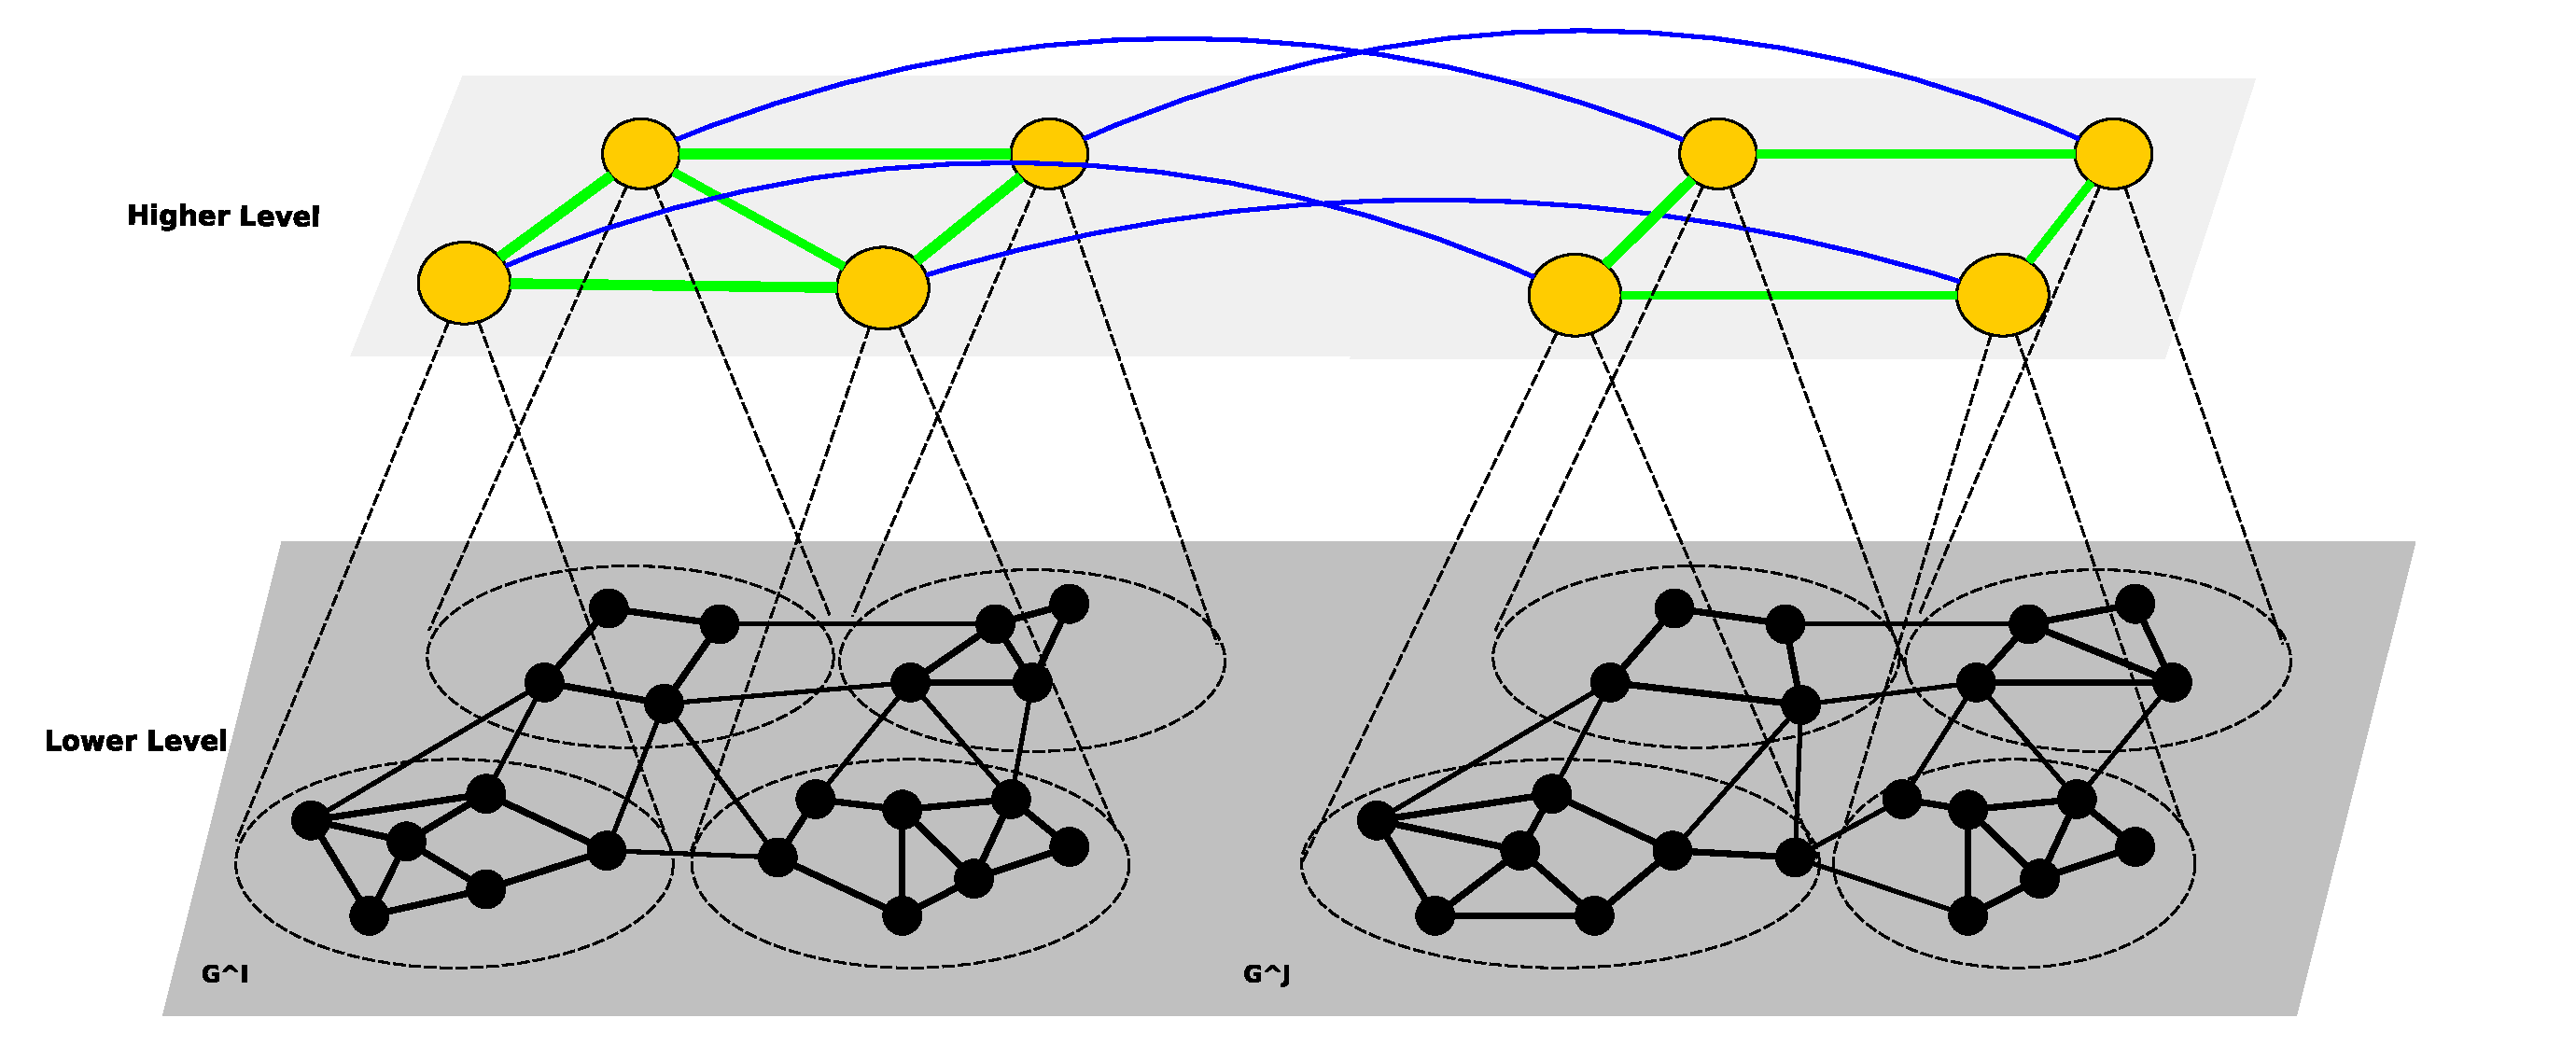
\includegraphics[scale=0.35]{chapter2/fig/twolevels2.pdf}
	\caption{Two level framework for graph matching} \label{fig:2levels}
\end{figure}

We return now back to the case of two graphs $G^I=(V^I,E^I,D^I)$ and $G^J=(V^J,E^J,D^J)$, which we want to match. 
For each of them we build an anchor graph $A^I=(V^{Ia},E^{Ia})$ and $A^J=(V^{Ja},E^{Ja})$ respectively.
Now instead of matching graphs $G^I$ and $G^J$ directly on the lower level, we may want to match first the corresponding anchor graphs. Matches between anchor nodes give us correspondences between underlying subgraphs. After that, we can perform graph matching for each pair of subgraphs completely independently. A union of local solutions from single subgraph matching problems gives us a solution of initial problem. 

Why this approach can be better than direct one? As we seen from the previous section the complexity of the considering graph matching problem depends highly on the size if initial graphs. Constructed anchor graphs are however several time smaller than initial graphs, which means, the matching algorithm on the anchor level can be performed much faster then on the lower level. The same holds for matching between the subgraphs.
%If $C(n)$ is complexity of a graph matching algorithm with $n$ possible correspondences.
Obviously, the accuracy of such two level matching approach depends heavily on the partition of the initial graphs into subgraphs and on the matching quality of the anchor graphs. To make the described two level approach more robust again graph partitioning we suggest to perform described steps iteratively till convergence of the objective function~\eqref{eq:gQAP1_2}. On each iteration we want to use an obtained matching between two graphs to correct graph partitioning. 

In the following we describe in details the single steps of our approach: initial graph construction, graph partitioning, graph matching algorithm on both levels, as well as an update rules of graph partitioning from a previous level.
\FloatBarrier
% ------------------------------------------------------------------------------------------------------------
% ---------------------------------------        HLG Construction
\subsection{Anchor Graph Construction}

A problem of anchor graph construction given an initial graph $G^I=(V^I,E^I,D^I)$ turns straight forward into problem of partitioning the graph $G^I$. During our work on this thesis we tried out different strategies for clustering nodes of a given graph. Here we present those, which were more suitable for our matching framework, however generally an arbitrary algorithm for graph partitioning can be used.
\subsubsection{Using grid}	
The first algorithm we describe is the most simple one. It uses a grid with fixed number of rows $r$, columns $c$ and a cell width $w$. The grid is placed over the graph $G$. Nodes, that are captured by a same grid cell belong to one cluster. Obviously, the number of clusters is equal to $r\times c$. Clusters, whose cells have a common edge are connected by an edge.
	                                                 
\subsubsection{Algorithms based on node merge}	                         
To construct an anchor graph $A$ with fixed number $m$ of anchors from a given fine graph $G$ we adopted coarsening phase from multi-level graph partition algorithms \cite{Chevalier09_GP, Safro2012_GC, Karypis95_GP, Hendrickson1995}.
Such algorithms have three phases: 
\begin{enumerate}
	\item graph coarsening phase, where one creates a hierarchy of graphs by successive merging of nodes in graph on previous stage starting with initial graph;
	\item graph partition stage, where the partition problem is solved exact on the coarsest level;
	\item refinement phase, where solution of the coarsest level is interpolated through all levels of the hierarchy until the initial graph.
\end{enumerate}
There are several types of graph coarsening algorithms. In our work we used so-called strict aggregation scheme (\textbf{SAG}) \cite{Chevalier09_GP}, which groups nodes of $G$ in \emph{disjoint} subsets based on the strength of the edges between them. 

We implemented two SAG based algorithms: Heavy Edge Matching (\textbf{HEM}) and Light Edge Matching (\textbf{LEM})~\cite{Chevalier09_GP}. Both algorithms visit nodes of the $G$ in random order and construct a \emph{matching} $M$ of the graph. A selected node $v_i\in V(G)\setminus V(M)$ is matched to a node $v\prime\in V(G)\setminus V(M)$ in $M$, if $s_{vv\prime} = \max_{u\in N(v)} s_{vu}$ in case of HEM and
$s_{vv\prime} = \min_{u\in N(v)} s_{vu}$ in case of LEM. Here, $N(v)$ denotes the neighborhood of $v$, $V(M)$ the set of matched nodes and $s$ the strength of an edge. In case of LEM $s_{ii\prime} = l_{ii\prime}$ and in case of HEM $s_{ii\prime} = exp(-\frac{l_{ij}}{\sigma^2_{s}})$.

The edges in $M$ will be contracted, i.e.\ their endpoints will be replaced with a new node, that lies in the middle of a contracted edge and is connected to all neighbors of its endpoints.

It is clear, that one iteration of HEM or LEM reduces the number of nodes in $G$ at most by $\lfloor\frac{n}{2} \rfloor$ nodes. To get an coarse graph with $m$ nodes the coarsening algorithm should be repeated several times.

Obtained at the end coarse graph is the desired anchor graph $A$ of $G$. 

\subsection{Anchor graph matching}

Assume, that for each of two given lower level graphs $G^I = (V^I, E^I, D^I)$ and $G^J=(V^J, E^J, D^J)$ we built the corresponding anchor graphs  $A^I=(V^{Ia},E^{Ia}, U^{Ia})$ and $A^J=(V^{Ja},E^{Ja},U^{Ja})$. 

We define the length of edges between two anchors $a_k$, $a_k\prime$ as a mean of distances between nodes in the corresponding subgraphs $G_k$ and $G_{k\prime}$. With other words:
\begin{equation} L_{kk\prime} = \median_{v_i\in G_k, v_{i\prime}\in G_{k\prime}} l_{ii\prime} \end{equation}
Based on this definition we use the same formula for \emph{edge similarity} between anchors as we set it for the lower level graphs (see Eq.\ref{eq:s_e}):
\begin{equation} 
s^A_E(e_{kk\prime}, e_{pp\prime}) = exp(-\frac{(L_{kk\prime} - L_{pp\prime})^2}{\sigma^2_{s}})
\label{eq:s_e_A}
\end{equation}
where $L_{kk\prime}$, $L_{pp\prime} $ are the lengths of edges $e_{kk\prime}\in E^{Ia}$ and $e_{pp\prime}\in E^{Ja}$ respectively.

To measure \emph{similarity between the anchors} we  define two different descriptors of an anchor $a$.

The first descriptor $d_1(a)$ should measure the similarity of node descriptors in corresponding subgraphs. For this purpose we adopted \emph{Bag Of Feature Model} \ToDo{ref}: we built a common dictionary based on the descriptors in $D^I$ and $D^J$ and define $d_1(a)$ as a histogram of "codewords" in corresponding subgraphs.

The second descriptor $d_2(a)$ should describe the structure similarity of subgraphs. We define $d_2(a)$ as a set of histograms $\{d_2(a,v)\}$ of the nodes $v$ in the underlying subgraph of the anchor $a$. The histograms of nodes have the fix number of bins $b$ and represent a distribution of the length of the subgraph edges inside a small circle region around each node. 

The similarity value between two anchors can be calculated now based on the first or second type of anchor descriptors by calculation of a distance between histograms based on $\chi^2$ statistic test \cite{Weken2004_ChiSqTest}:
\begin{equation}
s^A_1(a_k, a_p) = \sum_{b_i\in B}\frac{(d_1(a_k)-d_1(a_p))^2}{(d_1(a_k)+d_1(a_p))}
\end{equation}

\begin{equation}
s^A_2(a_k, a_p) = \frac{1}{|V(G_k)|}\frac{1}{V(G_p)|}\sum_{v\in V(G_k)}\sum_{u\in V(G_p)} \big(\sum_{b_i\in B}\frac{(d_2(a_k,v)-d_2(a_p,u))^2}{(d_2(a_k,v)+d_2(a_p,u))}\big)
\end{equation}

In our framework we use a combination of both anchor similarity functions:
\begin{equation}
s^A(a_k, a_p) = s_1(a_k, a_p)+s_2(a_k, a_p) 
\end{equation}

% ------------------------------------------------------------------------------------------------------------
% ---------------------------------------        LLG Construction
\subsection{Subgraph matching}
Given two corresponding subgraphs $G^I_{k_1}=(V^I_{k_1},E^I_{k_1},D^I_{k_1})$ and $G^J_{k_2}=(V^J_{k_2},E^J_{k_2},D^J_{k_2})$
%In our work we concentrate ourself on the task of finding feature correspondences between two images. Features are collected using such popular feature detectors as SIFT~\cite{Lowe2004}, MSER~\cite{MSER}. Extracted features from two images define the sets of nodes $V^I$, $V^J$ of the graphs $G^I$, $G^J$ respectively. As node attributes $D^I$, $D^J$ we used SIFT descriptors~\cite{Lowe2004} with fixed orientation and scale. 
%The nodes of the graphs are connected vie edges with their $k$ nearest neighbors.

To calculate the affinity matrix $S$ between two lower level graphs  $G^I$, $G^J$ or their subgraphs we need to define similarity functions between nodes and edges. Similarity of two nodes $v_i\in V^I, u_j\in V^J$ is equal to \emph{cosine similarity} of their descriptors.
For the pairwise edge similarity we used the same formula as in \cite{Cho2014_Haystack, Suh_CVPR2015}, i.e.\ 
\begin{equation}
s_E(e_{ii\prime}, e_{jj\prime}) = exp(-\frac{(l_{ii\prime} - l_{jj\prime})^2}{\sigma^2_{s}})
\label{eq:s_e}
\end{equation}
where $l_{ii\prime}$, $l_{jj\prime} $ are the lengths of edges $e_{ii\prime}\in E^I$ and $e_{jj\prime}\in E^J$ respectively.

% ------------------------------------------------------------------------------------------------------------
% ---------------------------------------        Matcing algorithm
\subsection{Matching Algorithm}

Generally, it is possible to use in our approach arbitrary graph matching algorithm for finding correspondences between anchors (higher level) and nodes (lower level). However we selected \emph{Reweighted Random Walks Method} (\textbf{RRWM})~\cite{Cho2010_RRWM}, as it shows high matching accuracy ($64.01\%$ in average) and is fast. Additionally, it	 suits well for finding common subgraph of two graphs in presence of outliers.

Important is, that the algorithm solves relaxed version of the initial problem (see section \ref{sec:prob_stat}), where constraints (\ref{QIP:3}),(\ref{QIP:4}) are dropped and the integrality constrain (\ref{QIP:2}) is replaced with $x\in \{0,1\}^{n_1n_2}$. We used \emph{greedy mapping} analog to \cite{Leordeanu2005}, instead of Hungarian algorithm used by the authors for discretization of continues solutions.

% ------------------------------------------------------------------------------------------------------------
% ---------------------------------------        Level connection
\subsection{Connection between two levels}
Assume, we solved the GMP on the higher level. That means, we know pairs of correspondences between the anchor nodes: $m^a = \{(a_k, a_p)\}, a_i\in V^{Ia}, a_p\in V^{Ja}$. Since each anchor represents a subgraph of the initial graph, $m^a$ defines at the same time the correspondences between the subgraphs of the initial graphs $G^I$ and $G^J$. Solution of the $GMP$ for each pair of the subgraphs gives us the desirable correspondences between the nodes of the original graphs ($m = \{(v_i, v_j)\}, v_i\in V^{I}, v_j\in V^{J}$).

As we already mentioned above, the quality of the resulting solution $m$ depends in our framework not only on the quality of the graph matching algorithm, but also on the graph partitioning algorithm. The Fig.~\ref{fig:badpartition} shows, that by the fixed partition the matching results will be very pure for all possible matches of the anchors.

\begin{figure}
	\centering
	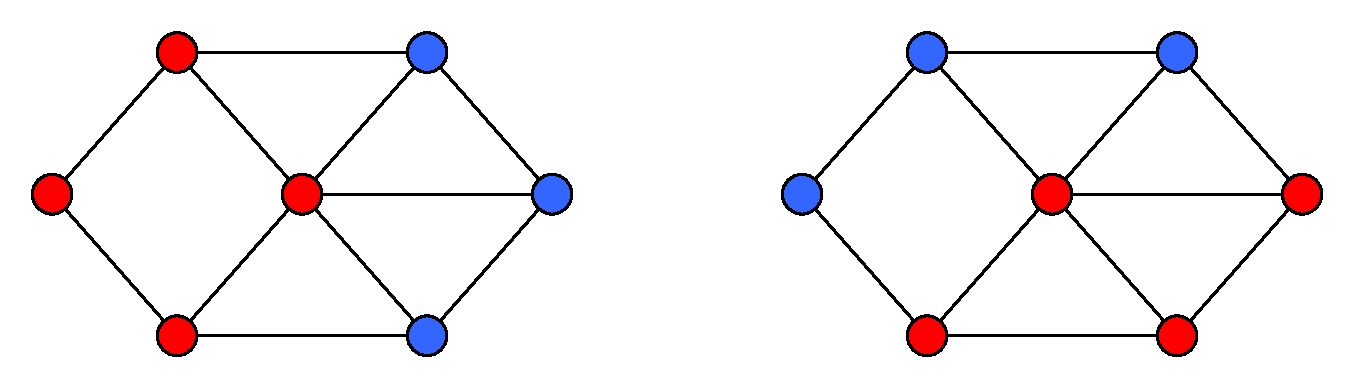
\includegraphics[scale=0.35]{chapter2/fig/badpartition.pdf}
	\caption{Example of bad partition of two equal graphs into two subgraphs} \label{fig:badpartition}
\end{figure}


To cope with this problem, we present an \emph{iterative approach}, where the subgraphs of the initial graphs are allowed to exchange nodes based on the solution $m$ after each iteration of two-level graph matching algorithm. Exchanging rules are based on the affine transformations assigned to each matched pair of the subgraphs.

We consider two matched subgraphs $G^I_k=(V^I_k, E^I_k, D^I_k)$ and  $G^J_p=(V^J_p, E^J_p, D^J_p)$. Based on the matching between the nodes of this pair we apply \emph{RANSAC}~\cite{RANSAC} to estimate two \emph{affine transformations} $T_{kp}:V^I_k\rightarrow V^J_p$ and $T_{pk}:V^J_p\rightarrow V^I_k$. From this two transformations we select the one with smaller transformation error. The transformation error is defined as follows. For each node $v_i\in V^I_k$ we calculate the error between its matched node $m(v_i) = v_j\in V^J_p$ and its projection $T_{kp}(v_i)$: 
\begin{equation} \label{eq:err_v}
err(v_i) = \|T_kp(v_i) - m(v_i)\|_{l_2}
\end{equation}
The error of the estimated affine transformation $T_{kp}$ (analog for  $err(T_{pk})$) is then defined as
\begin{equation} \label{eq:err_T}
err(T_{kp}) = \median_{v_i\in V^I_k}err(v_i)
\end{equation}

For the transformation with the smallest error we calculate its inverse transformation and associate both of them with the subgraph match $(a_k, a_p)$. For simplicity we preserve the notation $T_{kp}$ and $T_{pk}$ for the transformations related to the subgraph match $(a_k, a_p)$.

In this way we can associate to each subgraph pair with more than $3$ node correspondences \footnote{we need at least $3$ pair of correspondences to be able to estimate an affine transformation} the estimated affine transformation of their nodes.

\textit{Rule $1$}

If the transformation describes well the matching between the subgraphs nodes (i.e.\ the transformation error~\ref{eq:err_T} is small), then we include nodes near $T_{kp}(V^I)$, $T_{pk}(V^J)$ in corresponding subgraph with the confidence value equal to $e^{-\min(err(T_{kp}), err(T_{pk}))}$. If one node was selected by several subgraphs, it will be included in the subgraph with the biggest associated confidence value.

\textit{Rule $2$}

If there are subgraph with less then $3$ nodes, we shift this nodes to the subgraphs of their nearest neighbors. For this nodes $err(v)=M$ (see Eq.~\ref{eq:err_v}), where $M$ is some big constant. 

The described approach for subgraph reorganization is summarized in Algorithm~\ref{alg:update_subgraphs}.

\vspace{20pt}
\begin{algorithm}[H]
	\KwIn{ correspondence matrices between nodes of the initial\\
		   \hspace{45pt}graphs and anchors: $U^{Ia}$, $U^{Ja}$\\
		   \hspace{45pt}list of matches between the subgraphs: $m^a = \{(a_k, a_p)\}$;\\
   		   \hspace{45pt}list of estimated affine transformations for each matched \\
   		   \hspace{45pt}pair: $\{(T_{kp}, T_{pk})\}$ }
	\KwOut{new correspondence matrices $\hat{U}^{Ia}$, $\hat{U}^{Ja}$}
	\nl define subgraphs of the initial graphs based on the correspondence \\
	matrices $U^{Ia}$, $U^{Ja}$: $\{G^I_k\}$ and  $\{G^J_p\}$ \\
	\nl $\hat{U}^{Ia} = \frac{1}{2}U^{Ia}$, $\hat{U}^{Ja} = \frac{1}{2}U^{Ja}$ \\
	\nl \ForEach{matched subgraph pair $(a_k, a_p)$}
			{\eIf{$\left|V^I_k\right|\ge 3$ \textbf{AND} $\left|V^J_p\right|\ge 3$}
				{ 
			      $err = \min(err(T_{kp}), err(T_{pk}))$ \tcp*{ see equations \ref{eq:err_v}, \ref{eq:err_T}}
 			      \If{
 			      	 $\left| err\right| < \epsilon $}   %\tcp*{ matching is reliable}
			         {
%			          \tcc{ confidence of the included node to belong to considering subgraphs equals $\exp(-err)$ }
			          $\hat{U}^{Ja}(v, a_p) = \exp(-err)$ for $v\in T_{kp}(V^{I}_k)$ \\
   		 	          $\hat{U}^{Ia}(v, a_k) = \exp(-err)$ for $v\in T_{pk}(V^{J}_p)$ \\
   		 	         }
   		 	    }
    		 	{shift nodes of too small subgraphs into subgraphs, their nearest neighbors belong to} 
		    }			
	\nl  set in each row of  $\hat{U}^{Ia}$($\hat{U}^{Ja}$) the maximum element to $1$ and all other to $0$\\
	\Return $\hat{U}^{Ia}$, $\hat{U}^{Ja}$
	
	\caption{UpdateSubgraphs}    \label{alg:update_subgraphs}
\end{algorithm}

\FloatBarrier

\subsubsection{Simulated Annealing \textbf{SM}}

After some experiments we found out, that the iterative aproach based on the two-level graph matching and the Algorithm~\ref{alg:update_subgraphs} can stay trapped in local optima.
To cope with this we use additionally ideas of the \emph{Simulated Annealing}.

We consider each of the two graphs separately. In each iteration \emph{after application of the Algorithm~\ref{alg:update_subgraphs}} we randomly try to shift a node to one of its three nearest anchors. The energy state of the system is defined as $E = \sum_{v\in V}err(v)$ (see Eq.~\ref{eq:err_v}). After one node was shifted, the new energy state $E^{new}$ is calculated. Wenn $E^{new}<E$ the shifted node stays in its new subgraph. Otherwise, the move is accepted with the probability $exp(-\frac{E^{new}-E}{T})$, where $T = 1/{it}$ is the current temperature of the system and depends on the iteration number $it$. 

\emph{Afterwards} we apply again the Algorithm~\ref{alg:update_subgraphs}. 


  \chapter{Evaluation results} \label{chapter:results}

In this chapter we explore the quality of the proposed two level graph matching framework (we call it further 2LevelGM) on synthetic and real examples. The quality is measured by the matching score and accuracy of an obtained solution together with the running time in seconds needed to find it. Note, that under accuracy we understand actually recall of the graph matching algorithms (i.e. number of correct detected matches divided by the number of all correct matches), as it is done in~\cite{Cho2014_Haystack,Cho2010_RRWM,Cho2012_ProgressiveGM,Duchenne2011,Rangarajan1996_GAGM,Leordeanu2005_SM,Leordeanu2009_IPFP}.
To rate the usefulness of 2LevelGM we provide a comparison study across different graph matching algorithms. All tests in this chapter have been executed on a computer with an Intel(R) Core(R) i5-3210M CPU 2.50GHz with $4$ cores unless otherwise specified. We implemented our framework in the software package MATLAB and used $2$ workers\footnote{For more details see~\url{http://mathworks.com/help/distcomp/parallel-pools.html}} to run 2LevelGM. The code was not optimized. The sources of additionally used libraries and algorithms for comparisons are referred directly in the text. To make the comparison between the algorithms fair we used in all cases the same greedy assignment algorithm~\cite{Leordeanu2005_SM} for discretization of an obtained continuous solution. We also included the initialization and discretization steps into the runtime measurement.

\section{Synthetic data}
For the first set of tests we adopted a commonly used approach for evaluation of graph matching algorithms on two synthetic generated sets of points (see \cite{Cho2014_Haystack}, \cite{Cho2010_RRWM}, \cite{Leordeanu2009_IPFP}). 
For this purpose one generates first a set $V^I\subset\mathbb{R}^2$ of $n_1$ standard normally distributed points on a plane: $V^I=\{v_i=(x_i,y_i)|x_i\sim\mathcal{N}(0,1),y_i\sim\mathcal{N}(0,1),i=1,\dots,n_1\}$. In a second step $V^J$ is generated, which represents a distorted copy of the first set with $\bar{n}$ additional normally distributed points. The distortion is achieved by adding a normally distributed noise with zero mean and a variance $\sigma^2$ to the coordinates of the points in $V^I$. 
%The parameter $\sigma$ expresses the deformation in the second set $V^J$.
This means, that the set $V^J$ consists of $n_2=n_1+\bar{n}$ nodes, where $n_1$ points have a unique pair in $V^I$ and are called inliers, whereby the other $\bar{n}$ points are outliers. The task is to find correspondences between points in the two sets, which obviously can be considered as a graph matching problem. For that we consider two fully connected graphs $G^I$ and $G^J$ with the nodes defined by the points in $V^I$ and $V^J$ respectively. We assume, that the graphs do not have attributes and each node in the first graph can be theoretically matched to each node in the second graph.

For the evaluation of our graph matching framework we follow the setup of the synthetic point set tests from the papers~\cite{Cho2014_Haystack} and \cite{FastPFP} and formulate four different kinds of tests. In the first test we set the number of outliers $\bar{n}$ to zero and vary only the deformation noise $\sigma^2$. In the second test, we do not have a deformation noise ($\sigma^2=0$) and compare the behavior of the different graph matching algorithms in case of a increasing number of outliers $\bar{n}$. In the third test, we perform the second test in presence of deformation in the second graph. For this we fix $\sigma^2= 0.03$ and increase iteratively the number of outliers $\bar{n}$. Finally, in the fourth test we consider again two graphs with the same size, but omit randomly $\theta$ percentage of edges in both graphs with increasing $\theta$. 
For performing the tests we adopted the supplemental MATLAB code provided by Minsu Cho et al. in their paper~\cite{Cho2014_Haystack,code_MPM}. For simplicity we combine the described tests together in a first group of tests. %and present results of its test below.We combine the described tests in one group and perform further a comparison of graph matching algorithms on two such groups, that differ in the size of considered graphs inside them. 

The first graphs we consider are relatively small: $100-150$ nodes. The main reason for using small graphs is to compare the 2LevelGM with the following well known methods: MPM~\cite{Cho2014_Haystack}, RRWM~\cite{Cho2010_RRWM}, SM~\cite{Leordeanu2005_SM} and IPFP~\cite{Leordeanu2009_IPFP}\footnote{We used the implementation of those algorithms provided in~\cite{code_MPM}.}. The selection of the graph size was determined by application examples of the corresponding algorithms provided in the mentioned publications. To our best knowledge, those algorithms has not been applied directly to graphs with more than $150$ nodes each without additional problem simplifications (for example reduction of the set of possible correspondences, which is difficult to achieve for non-attributed graphs). This restriction on the size of the graphs is determined mainly by the size of the dense affinity matrix $S$, which is used by all algorithms. The matrix $S$ is calculated in all cases using Eq.~\eqref{eq:edge_sim1_2} with $\sigma_s^2=0.15$, where the value of the parameter $\sigma_s^2$ is chosen according to the proposition made in~\cite{Cho2010_RRWM}. To calculate affinity matrix on the anchor level we use $\sigma_s^2=10$. 

Since our initial graphs $G^I$ and $G^J$ are not attributed, we first consider the formulation of 2LevelGM with non-attributed anchors graphs. The similarities between anchors are calculated in this case based on the matching score of the underlying subgraphs (see chapter~\ref{anchorGraphMatching}). For the initialization of the initial subgraphs we use the grid method (see chapter~\ref{subgraphInit}) with $2\times 2$ cells. The average matching results of $10$ runs in the four defined tests are illustrated in Figs.~\ref{fig:synTest1_ver433}-\ref{fig:synTest4_ver433}. The vertical bars at each point show the standard deviation of the measured mean value (accuracy, matching score and running time) for the corresponding problem setting.
% -----------------------------  Version 4.3.3    -------------------------------
\begin{figure}
	\begin{subfigure}[b]{0.33\textwidth}
		\centering
		\includegraphics[scale=0.25]{"chapter3/fig/SyntheticTest/no_descr/Results_v4.3.3/Test2/accuracy_avg10t"} 
	\end{subfigure}
	\begin{subfigure}[b]{0.33\textwidth}
		\centering
		\includegraphics[scale=0.25]{"chapter3/fig/SyntheticTest/no_descr/Results_v4.3.3/Test2/score_avg10t"} 
	\end{subfigure} 
	\begin{subfigure}[b]{0.32\textwidth}
		\centering
		\includegraphics[scale=0.25]{"chapter3/fig/SyntheticTest/no_descr/Results_v4.3.3/Test2/time_summary_avg10t"} 
	\end{subfigure} 
	\caption[Performance of the 2LevelGM with non-attributed anchor graphs on synthetic data (test $1$)]{Performance of the 2LevelGM with non-attributed anchor graphs on synthetic data: test $1$ ($n_1=100$, $\bar{n}=0$, $\theta=100\%$)}
	\label{fig:synTest1_ver433}
\end{figure}
%\vspace{-20pt}
\begin{figure}
	\begin{subfigure}[b]{0.33\textwidth}
		\centering
		\includegraphics[scale=0.25]{"chapter3/fig/SyntheticTest/no_descr/Results_v4.3.3/Test3/accuracy_avg10t"} 
	\end{subfigure}%% 
	\begin{subfigure}[b]{0.33\textwidth}
		\centering
		\includegraphics[scale=0.25]{"chapter3/fig/SyntheticTest/no_descr/Results_v4.3.3/Test3/score_avg10t"} 
	\end{subfigure} 
	\begin{subfigure}[b]{0.33\textwidth}
		\centering
		\includegraphics[scale=0.25]{"chapter3/fig/SyntheticTest/no_descr/Results_v4.3.3/Test3/time_summary_avg10t"} 
	\end{subfigure} 	
	\caption[Performance of the 2LevelGM with non-attributed anchor graphs on synthetic data (test $2$)]{Performance of the 2LevelGM with non-attributed anchor graphs on synthetic data: test $2$ ($n_1=100$, $\bar{n}\in[0,50]$, $\sigma^2=0$, $\theta=100\%$)}
	\label{fig:synTest2_ver433}
\end{figure}
%\vspace{-20pt}
\begin{figure}
		\begin{subfigure}[b]{0.33\textwidth}
			\centering
			\includegraphics[scale=0.25]{"chapter3/fig/SyntheticTest/no_descr/Results_v4.3.3/Test1/accuracy_avg10t"} 
		\end{subfigure}%% 
		\begin{subfigure}[b]{0.33\textwidth}
			\centering
			\includegraphics[scale=0.25]{"chapter3/fig/SyntheticTest/no_descr/Results_v4.3.3/Test1/score_avg10t"} 
		\end{subfigure} 
		\begin{subfigure}[b]{0.33\textwidth}
			\centering
			\includegraphics[scale=0.25]{"chapter3/fig/SyntheticTest/no_descr/Results_v4.3.3/Test1/time_summary_avg10t"} 
		\end{subfigure} 	
	\caption[Performance of the 2LevelGM with non-attributed anchor graphs on synthetic data (test $3$)]{Performance of the 2LevelGM with non-attributed anchor graphs on synthetic data: test $3$ ($n_1=100$, $\bar{n}\in[0,50]$, $\sigma^2=0.03$, $\theta=100\%$)}
	\label{fig:synTest3_ver433}
\end{figure}
%\vspace{-20pt}
\begin{figure}
		\begin{subfigure}[b]{0.33\textwidth}
			\centering
			\includegraphics[scale=0.25]{"chapter3/fig/SyntheticTest/no_descr/Results_v4.3.3/Test4/accuracy_avg10t"} 
		\end{subfigure}%% 
		\begin{subfigure}[b]{0.33\textwidth}
			\centering
			\includegraphics[scale=0.25]{"chapter3/fig/SyntheticTest/no_descr/Results_v4.3.3/Test4/score_avg10t"} 
		\end{subfigure} 
		\begin{subfigure}[b]{0.33\textwidth}
			\centering
			\includegraphics[scale=0.25]{"chapter3/fig/SyntheticTest/no_descr/Results_v4.3.3/Test4/time_summary_avg10t"} 
		\end{subfigure} 	
	\caption[Performance of the 2LevelGM with non-attributed anchor graphs on synthetic data (test $4$)]{Performance of the 2LevelGM with non-attributed anchor graphs on synthetic data: test $4$ ($n_1=n_2=100$, $\sigma^2=0$)}
	\label{fig:synTest4_ver433}
\end{figure}
%\FloatBarrier
%-------------------------------------------------------------------------------

From this results one can see that the SM algorithm has the worst matching quality in all cases. 2LevelGM performs little bit unstable, which is indicated by a relatively high standard deviation compared with other algorithms. For this reason its average performance (objective score and accuracy) of 2LevelGM is a little bit lower than the one of IPFP and RRWM, although in individual runs 2LevelGM is not worse. Additionally the running time of 2LevelGM is slower as for IPFP and RRWM. However this is expected, because without anchor attributes 2LevelGM performs graph matching using RRWM on each pair of subgraphs. Although those subgraphs are smaller than the initial graphs, the overall complexity of this procedure for relative small graphs $G^I,G^J$ is higher compared to the one for direct application of RRWM. The best matching results are achieved in three of four tests by the MPM, which is also the slowest algorithm. However, it is outperformed by 2LevelGM in the first test (Fig.~\ref{fig:synTest1_ver433}) with significantly smaller time demand\footnote{The used implementations of 2LevelGM, SM and IPFP are purely MATLAB implementations, whereby some steps of MPM and RRWM were written using $C++$. This makes the comparison of the running time between algorithms difficult.}.

Below we present the results of testing on the first group of tests using 2LevelG with attributed anchor graphs. For this purpose we use the attributes, that capture geometrical structure of the subgraphs (see chapter~\ref{anchorGraphMatching}). We set the size of used histograms to $35$ bins and the radius $R$ of the circle region around each node to $2$. The results of the comparison are presented in Figs.~\ref{fig:synTest1_descr_ver433}-\ref{fig:synTest4_descr_ver433}. One can directly see the improved performance time of the 2LevelGM algorithm in all tests. The proposed algorithm also shows a more stable performance in the second test. 
%, which practically solves subgraph the isomorphism problem.
On the other side, the algorithm seems to be more susceptible to graph deformations (see Figs.~\ref{fig:synTest1_descr_ver433}, \ref{fig:synTest4_descr_ver433}). The reason for this is in the selected anchor attributes, that are not sufficiently robust against deformations in the length of edges.

% -----------------------------  Version 4.3.3    -------------------------------
\begin{figure}[h]
	\begin{subfigure}[b]{0.33\textwidth}
		\centering
		\includegraphics[scale=0.25]{"chapter3/fig/SyntheticTest/descr/Results_v4.3.3/Test2/accuracy_avg10t"} 
	\end{subfigure}
	\begin{subfigure}[b]{0.33\textwidth}
		\centering
		\includegraphics[scale=0.25]{"chapter3/fig/SyntheticTest/descr/Results_v4.3.3/Test2/score_avg10t"} 
	\end{subfigure} 
	\begin{subfigure}[b]{0.31\textwidth}
		\centering
		\includegraphics[scale=0.25]{"chapter3/fig/SyntheticTest/descr/Results_v4.3.3/Test2/time_summary_avg10t"} 
	\end{subfigure} 
	\caption[Performance of the 2LevelGM with attributed anchor graphs on synthetic data (test $1$)]{Performance of the 2LevelGM with attributed anchor graphs on synthetic data: test $1$ ($n_1=100$, $\bar{n}=0$, $\sigma^2=0$)}
	\label{fig:synTest1_descr_ver433}
\end{figure}
%\vspace{-25pt}
\begin{figure}[h]
	\begin{subfigure}[b]{0.33\textwidth}
		\centering
		\includegraphics[scale=0.25]{"chapter3/fig/SyntheticTest/descr/Results_v4.3.3/Test3/accuracy_avg10t"} 
	\end{subfigure}%% 
	\begin{subfigure}[b]{0.33\textwidth}
		\centering
		\includegraphics[scale=0.25]{"chapter3/fig/SyntheticTest/descr/Results_v4.3.3/Test3/score_avg10t"} 
	\end{subfigure} 
	\begin{subfigure}[b]{0.33\textwidth}
		\centering
		\includegraphics[scale=0.25]{"chapter3/fig/SyntheticTest/descr/Results_v4.3.3/Test3/time_summary_avg10t"} 
	\end{subfigure} 	
	\caption[Performance of the 2LevelGM with attributed anchor graphs on synthetic data (test $2$)]{Performance of the 2LevelGM with attributed anchor graphs on synthetic data: test $2$ ($n_1=100$, $\bar{n}\in[0,50]$, $\sigma^2=0$, $\theta=100\%$)}
	\label{fig:synTest2_descr_ver433}
\end{figure}
%\vspace{-25pt}
\begin{figure}[h]
		\begin{subfigure}[b]{0.33\textwidth}
			\centering
			\includegraphics[scale=0.25]{"chapter3/fig/SyntheticTest/descr/Results_v4.3.3/Test1/accuracy_avg10t"} 
		\end{subfigure}%% 
		\begin{subfigure}[b]{0.33\textwidth}
			\centering
			\includegraphics[scale=0.25]{"chapter3/fig/SyntheticTest/descr/Results_v4.3.3/Test1/score_avg10t"} 
		\end{subfigure} 
		\begin{subfigure}[b]{0.33\textwidth}
			\centering
			\includegraphics[scale=0.25]{"chapter3/fig/SyntheticTest/descr/Results_v4.3.3/Test1/time_summary_avg10t"} 
		\end{subfigure} 	
	\caption[Performance of the 2LevelGM with attributed anchor graphs on synthetic data (test $3$)]{Performance of the 2LevelGM with attributed anchor graphs on synthetic data: test $3$ ($n_1=100$, $\bar{n}\in[0,50]$, $\sigma^2=0.03$, $\theta=100\%$)}
	\label{fig:synTest3_descr_ver433}
\end{figure}
%\vspace{-25pt}
\begin{figure}[h]
		\begin{subfigure}[b]{0.33\textwidth}
			\centering
			\includegraphics[scale=0.25]{"chapter3/fig/SyntheticTest/descr/Results_v4.3.3/Test4/accuracy_avg10t"} 
		\end{subfigure}%% 
		\begin{subfigure}[b]{0.33\textwidth}
			\centering
			\includegraphics[scale=0.25]{"chapter3/fig/SyntheticTest/descr/Results_v4.3.3/Test4/score_avg10t"} 
		\end{subfigure} 
		\begin{subfigure}[b]{0.33\textwidth}
			\centering
			\includegraphics[scale=0.25]{"chapter3/fig/SyntheticTest/descr/Results_v4.3.3/Test4/time_summary_avg10t"} 
		\end{subfigure} 	
	\caption[Performance of the 2LevelGM with attributed anchor graphs on synthetic data (test $4$)]{Performance of the 2LevelGM with attributed anchor graphs on synthetic data: test $4$ ($n_1=n_2=100$, $\sigma^2=0.00$)}
	\label{fig:synTest4_descr_ver433}
\end{figure}
% --------------------------------------------------------------------------------

To test the performance of our framework on bigger graphs we performed another group of tests and compare 2LevelGM with the PATH~\cite{Zazlavskiy2008_PATH}\footnote{\url{http://cbio.ensmp.fr/graphm/}} and GLAG~\cite{Fiori2013_GLAG}\footnote{\url{http://www.fing.edu.uy/~mfiori/}. We replaced the default maximal number of iterations ($30000$) with $1000$.} algorithms. In contrast to the graph matching problem formulation considered by 2LevelGM and previous algorithms the PATH and GLAG algorithms solve the minimization problem from Eq.~\eqref{eq:QAP1}. Consequently they do not work with the affinity matrix $S$ and can therefore be directly applied to bigger graphs without the necessity to reduce the set of possible candidate matches. The result of the comparison in one run can be seen in Figs.~\ref{fig:synTest1_bigGraphs_ver433}-\ref{fig:synTest3_bigGraphs_ver433}\footnote{This group of tests was executed on a desktop PC with an 2.67GHz Intel(R) Xeon(R) CPU with $4$ cores. $4$ MATLAB workers were used}. We do not provide averaged results for this set of tests due to their high computational demand. For this tests we used again a grid initialization method for 2LevelGM with $5\times 4$ cells.
\FloatBarrier

\begin{figure}[h] 
		\begin{subfigure}[b]{0.33\textwidth}
			\centering
			\includegraphics[scale=0.25]{"chapter3/fig/SyntheticTest_BigGraphs/descr/Results_v4.3.3/Test1/accuracy_avg1t"} 
		\end{subfigure}
		\begin{subfigure}[b]{0.33\textwidth}
			\centering
			\includegraphics[scale=0.25]{"chapter3/fig/SyntheticTest_BigGraphs/descr/Results_v4.3.3/Test1/score_avg1t"} 
		\end{subfigure} 
		\begin{subfigure}[b]{0.32\textwidth}
			\centering
			\includegraphics[scale=0.25]{"chapter3/fig/SyntheticTest_BigGraphs/descr/Results_v4.3.3/Test1/time_summary_avg1t"} 
		\end{subfigure} 	
	\caption[Performance comparison of 2LevelGM, GLAG and PATH on bigger graphs: test $1$]{Performance comparison of 2LevelGM, GLAG and PATH on bigger graphs ($\bar{n}=0$, $\sigma^2=0$, $\theta=100\%$)}
	\label{fig:synTest1_bigGraphs_ver433}
\end{figure}
\begin{figure}[h] 
		\begin{subfigure}[b]{0.33\textwidth}
			\centering
			\includegraphics[scale=0.25]{"chapter3/fig/SyntheticTest_BigGraphs/descr/Results_v4.3.3/Test2/accuracy_avg1t"} 
		\end{subfigure}
		\begin{subfigure}[b]{0.33\textwidth}
			\centering
			\includegraphics[scale=0.25]{"chapter3/fig/SyntheticTest_BigGraphs/descr/Results_v4.3.3/Test2/score_avg1t"} 
		\end{subfigure} 
		\begin{subfigure}[b]{0.32\textwidth}
			\centering
			\includegraphics[scale=0.25]{"chapter3/fig/SyntheticTest_BigGraphs/descr/Results_v4.3.3/Test2/time_summary_avg1t"} 
		\end{subfigure} 	
	\caption[Performance comparison of 2LevelGM, GLAG and PATH on bigger graphs: test $2$]{Performance comparison of 2LevelGM, GLAG and PATH on bigger graphs ($\bar{n}=0$, $\sigma^2=0.03$, $\theta=100\%$)}
	\label{fig:synTest2_bigGraphs_ver433}
\end{figure}
\begin{figure}[h] 
		\begin{subfigure}[b]{0.33\textwidth}
			\centering
			\includegraphics[scale=0.25]{"chapter3/fig/SyntheticTest_BigGraphs/descr/Results_v4.3.3/Test3/accuracy_avg1t"} 
		\end{subfigure}
		\begin{subfigure}[b]{0.33\textwidth}
			\centering
			\includegraphics[scale=0.25]{"chapter3/fig/SyntheticTest_BigGraphs/descr/Results_v4.3.3/Test3/score_avg1t"} 
		\end{subfigure} 
		\begin{subfigure}[b]{0.32\textwidth}
			\centering
			\includegraphics[scale=0.25]{"chapter3/fig/SyntheticTest_BigGraphs/descr/Results_v4.3.3/Test3/time_summary_avg1t"} 
		\end{subfigure} 	
	\caption[Performance comparison of 2LevelGM, GLAG and PATH on bigger graphs: test $3$]{Performance comparison of 2LevelGM, GLAG and PATH on bigger graphs ($\bar{n}=0$, $\sigma^2=0$, $\theta=90\%$)}
	\label{fig:synTest3_bigGraphs_ver433}
\end{figure}

All performed tests in this group can be considered as instances of the graph isomorphism problem in exact (Fig.~\ref{fig:synTest1_bigGraphs_ver433}) and inexact (Figs.~\ref{fig:synTest2_bigGraphs_ver433},~\ref{fig:synTest3_bigGraphs_ver433}) forms. We investigate the matching score, accuracy and running time of the graph matching algorithms as functions of number of nodes in the initial graphs.
In all cases the proposed two level graph matching framework outperforms both GLAG and PATH in objective score and especially in running time with one exception. This one is the running rime of the last iteration in Fig.~\ref{fig:synTest2_bigGraphs_ver433}. We consider it as an individual case and suppose, that an imbalanced graph partitioning of initial graphs causes the jump in the running time. Overall 2LevelGM shows a high matching accuracy in all three tests. Additionally we believe it is possible to improve the framework by solving instability issues, which we saw in previous cases. 
\FloatBarrier
% --------------------------------------------------------------------
% --------------------------------------------------------------------
\section{Real data tests}
In the following sections we use the developed two level graph matching algorithm for finding correspondences between features on a pair of images. To formulate this problem as a graph matching problem we use the standard approach settled in computer vision literature~\cite{Cho2010_RRWM,Cho2012_ProgressiveGM,FastPFP,Hancock_EM_SVD,Hancock_GM_SpectralPart}. For that we extract SIFT features~\cite{Lowe2004} of two images around keypoints, that were located using some feature detector (we used  MSER~\cite{MSER}). Given the extracted features of two images we construct two attributed graphs $G^I=(V^I,E^I,D^I)$ and $G^J=(V^J,E^J,D^J)$ for each image respectively. The nodes of those graphs are placed at the locations of the detected keypoints with their features as node attributes. To connect nodes via edges one can use Delaunay triangulation~\cite{Hancock_EM_SVD,Hancock_GM_SpectralPart}, nearest neighbors relations between nodes~\cite{Sanrom2012} or consider complete graphs~\cite{Cho2012_ProgressiveGM,Cho2014_Haystack}.

\subsection{Image affine transformation}
The first image set we consider can be seen as a synthetic data set of real images. It consists of image pairs, where one image in each pair is the same in all cases and the second image represent a rotated/shifted copy of the first one with additional Gaussian noise added to its pixels (see Fig.~\ref{fig:ImageTrafo_initGraphs}\footnote{The presented image of a church is taken from the SUN\cite{SUN} dataset (category "church outdoor").}). On this simple examples we want to demonstrate the work of the update rule inside 2LevelGM algorithm (see chapter~\ref{updateRule}).

\begin{figure}[h] 
		\begin{subfigure}[b]{0.3\textwidth}
			\centering
			\includegraphics[width=4cm]{"chapter3/fig/ImageTrafo/Img_pair1"} 
			\caption{}\label{fig:ImageTrafo_initGraphs_a}
		\end{subfigure}
		\begin{subfigure}[b]{0.3\textwidth}
			\centering
			\includegraphics[width=4cm]{"chapter3/fig/ImageTrafo/Img_pair2"} 
			\caption{}
		\end{subfigure} 
		\begin{subfigure}[b]{0.3\textwidth}
			\centering
			\includegraphics[width=4cm]{"chapter3/fig/ImageTrafo/Img_pair3"}
			\caption{}
		\end{subfigure} 	
		\begin{subfigure}[b]{0.5\textwidth}
			\centering
			\includegraphics[width=4cm]{"chapter3/fig/ImageTrafo/Img_pair4"} 
			\caption{}
		\end{subfigure} 
		\begin{subfigure}[b]{0.5\textwidth}
			\centering
			\includegraphics[width=4cm]{"chapter3/fig/ImageTrafo/Img_pair5"}
			\caption{}
		\end{subfigure} 	
	\caption[Synthetic image data set]{Synthetic image data set: first image~\cite{SUN} in each pair is a transformed copy of the second image with Gaussian noise added to its pixels. Keypoints are extracted on the second image in each pair using MSER feature detector~\cite{MSER} and inherited by the first image, edges between nodes are built using Delaunay triangulation procedure~\cite{Hancock_EM_SVD,Hancock_GM_SpectralPart}}
	\label{fig:ImageTrafo_initGraphs}
\end{figure}

\begin{figure} 
	\begin{center}
		\begin{subfigure}[t]{0.32\textwidth}
			\includegraphics[width=4cm]{"chapter3/fig/ImageTrafo/sIterations/It1"} 
			\caption{Iteration $1$}
		\end{subfigure}
		\begin{subfigure}[t]{0.32\textwidth}
			\includegraphics[width=4cm]{"chapter3/fig/ImageTrafo/sIterations/It2"} 
			\caption{Iteration $2$}
		\end{subfigure} 
		\begin{subfigure}[t]{0.32\textwidth}
			\includegraphics[width=4cm]{"chapter3/fig/ImageTrafo/sIterations/It3"}
			\caption{Iteration $3$}
		\end{subfigure} 	
		\begin{subfigure}[t]{0.33\textwidth}
			\includegraphics[width=4cm]{"chapter3/fig/ImageTrafo/sIterations/accuracy"}
			\caption{Accuracy\hspace{5pt}}
			\label{fig:ImageTrafo_sIterations_d}
		\end{subfigure} 
		\begin{subfigure}[t]{0.33\textwidth}
			\includegraphics[width=4cm]{"chapter3/fig/ImageTrafo/sIterations/score"}
			\caption{Matching score\hspace{5pt}}
			\label{fig:ImageTrafo_sIterations_e}
		\end{subfigure}
		\begin{subfigure}[t]{0.3\textwidth}
			\includegraphics[width=4cm]{"chapter3/fig/ImageTrafo/sIterations/gap"}
			\caption{Gap between current and optimal solutions}
			\label{fig:ImageTrafo_sIterations_f}
		\end{subfigure} 	
	\end{center}		
	\caption[Result of applying 2LevelGM to the image pair~\ref{fig:ImageTrafo_initGraphs_a}]{Result of applying 2LevelGM to the image pair~\ref{fig:ImageTrafo_initGraphs_a}. Nodes of the matched subgraphs have the same color.}
	\label{fig:ImageTrafo_sIterations}
\end{figure}

To create the anchor graphs we used the HEM coarsening algorithm (see Alg.~\ref{alg:HEM}) with a fixed number of anchors. Since the initial graphs are not big (the right image in each pair contains $152$ keypoints), we set the number of anchors to $3$ for all anchor graphs. In this case the subgraphs are big enough to guaranty a robust estimation of an affine transformation between them. The work of 2LevelGM is illustrated in Fig.~\ref{fig:ImageTrafo_sIterations} on the example of the first image pair (Fig.~\ref{fig:ImageTrafo_initGraphs_a}). The nodes in the matched subgraphs have the same color. One can see how the initial graph partition changes through the iterations, which leads to the improvement in both objective score and accuracy (see Figs.~\ref{fig:ImageTrafo_sIterations_d}-\ref{fig:ImageTrafo_sIterations_f}). Fig.~\ref{fig:ImageTrafo_sIterations_f} shows additionally the decrease of the gap $\frac{x_i-x_{\text{opt}}}{x_{\text{opt}}}$ between the optimal solution $x_{\text{opt}}$ and solution in the i-th iteration $x_i$. It is easy to see that three iterations are sufficient. Further iterations do not improve matching.

In Fig.~\ref{fig:ImageTrafo} we present the results from matching with 2LevelGM of all $5$ image pairs in comparison with the results obtained with the progressive graph matching algorithm (ProgGM)~\cite{Cho2012_ProgressiveGM}. %\ToDo{The last is an iterative algorithm, which starts with a set of candidate matches between nodes of the initial graphs and updates this set in each iteration by replacing some candidates with a better one. The selection of new candidates is based on the estimation of a homography between features of matched nodes.}
To make the comparison fair, we use in both methods the Eq.~\eqref{eq:edge_sim1_2} with $\sigma_s^2=0.15$ to calculate the affinity matrix for the initial graphs and their subgraphs. For the anchor graphs we use the same formula but with $\sigma^2_s=10$. The size of the set of initial candidate matches used by ProgGM is limited by $3000$ pairs. For the rest we use the default parameters of ProgGM suggested by the authors with RRWM as its graph matching module.

It is pleasant to see that 2LevelGM is able to find the absolutely correct matching for the whole set except one image pair and therefore shows better results in objective score and accuracy than ProgGM does. The result of matching of the last image pair is roughly the same for both algorithms. We notice that 2LevelGM is not able to improve graph partitioning further in this case, although some nodes from the true matches belonged to different subgraphs. Regarding the running time ProgGM is faster. However we should point out, that ProgGM directly stops as soon as the matching score does not increase any more. In contrast to that, our 2LevelGM has to make some additional iterations at the end to ensure that a local minimum is found. This is done intentionally, as we cannot make certain statement about the convergence of our framework.

\begin{figure}[h] \centering
		\begin{subfigure}[b]{0.33\textwidth}
			\centering
			\includegraphics[scale=0.35]{"chapter3/fig/ImageTrafo/anchor_descr/using_cpd_afftrafo/performance/accuracy1"} 
		\end{subfigure} 
		\begin{subfigure}[b]{0.33\textwidth}
			\centering
			\includegraphics[scale=0.35]{"chapter3/fig/ImageTrafo/anchor_descr/using_cpd_afftrafo/performance/score1"} 
		\end{subfigure}
		\begin{subfigure}[b]{0.32\textwidth}
			\centering
			\includegraphics[scale=0.35]{"chapter3/fig/ImageTrafo/anchor_descr/using_cpd_afftrafo/performance/time1"}
		\end{subfigure} 	
	\caption[Evaluation of 2LevelGM on the synthetic image dataset (see Fig.~\ref{fig:ImageTrafo_initGraphs})]{Evaluation of 2LevelGM on the synthetic image dataset (see Fig.~\ref{fig:ImageTrafo_initGraphs})}
	 \label{fig:ImageTrafo}
\end{figure}

\subsection{House dataset}
Our next data set is the well known CMU House sequence~\cite{CMUHouse} which consists of $111$ images of a toy house taken from different viewpoints. It was widely used for the evaluation of graph matching algorithms~\cite{Armiti2014,Hancock_ModalClusters,Cho2010_RRWM,Duchenne2011,FastPFP,Hancock_EM_SVD}. The provided ground truth~\cite{CMUHouse_GT} consists of $30$ feature points presented in all frames in the sequence. Due to that reason most authors considered for matching small graphs with $30$ nodes. By analogy with the previous dataset we used MSER to extract around $250$ keypoints on each image in the sequence with SIFT descriptors and use all of them to build the initial graphs to be matched. The provided ground truth is extrapolated to neighboring features in the same way it was done in~\cite{Cho2012_ProgressiveGM}\footnote{We set the radius of extrapolation to $10$.}. We perform matching between pairs of images spaced by $1$, $10$, $20$, \dots, $110$ frames. However we match at maximum $10$ image pairs for each gap (i.e. detachment between frames). Further we  analyze the averaged matching score, accuracy and running time of 2LevelGM, ProgGM and simple feature matching~\cite{Lowe2004} as functions of the sequence gap. Notice that the bigger the gap the stronger is the deformation between the object on two images and the more difficult is the matching problem. 

The results of matching can be seen in Figs.~\ref{fig:House_sol}-\ref{fig:House_ext_sol}. The difference between two provided groups of results lies in the post-processing step applied to the final solutions of all three algorithms in the second group. This post processing step is initially used only by ProgGM to extrapolate the obtained graph matching solution in the same way as it is done for the ground truth~\cite{Cho2012_ProgressiveGM}. This leads to the possibly not unique correspondences between node sets of initial graphs and, in our opinion, significantly increases the accuracy of the solution (compare images in Fig.~\ref{fig:sol_ext}). To make the comparison fairer we applied the same post-processing step also to the solutions of 2LevelGM and feature matching.

\begin{figure}[h] \centering
		\begin{subfigure}[b]{0.33\textwidth}
			\centering
			\includegraphics[scale=0.25]{"chapter3/fig/HouseSeq2/anchor_descr/using_cpd_afftrafo/solution/performance/accuracy"} 
		\end{subfigure} 
		\begin{subfigure}[b]{0.33\textwidth}
			\centering
			\includegraphics[scale=0.25]{"chapter3/fig/HouseSeq2/anchor_descr/using_cpd_afftrafo/solution/performance/score"} 
		\end{subfigure}
		\begin{subfigure}[b]{0.32\textwidth}
			\centering
			\includegraphics[scale=0.25]{"chapter3/fig/HouseSeq2/anchor_descr/using_cpd_afftrafo/solution/performance/time_summary"}
		\end{subfigure} 	
	\caption[Evaluation of 2LevelGM on the CMU House sequence]{Evaluation of 2LevelGM on the CMU House sequence: not extrapolated solution} \label{fig:House_sol}
\end{figure}

\begin{figure}[h] \centering
		\begin{subfigure}[b]{0.33\textwidth}
			\centering
			\includegraphics[scale=0.25]{"chapter3/fig/HouseSeq2/anchor_descr/using_cpd_afftrafo/ext_solution/performance/accuracy"} 
		\end{subfigure} 
		\begin{subfigure}[b]{0.33\textwidth}
			\centering
			\includegraphics[scale=0.25]{"chapter3/fig/HouseSeq2/anchor_descr/using_cpd_afftrafo/ext_solution/performance/score"} 
		\end{subfigure}
		\begin{subfigure}[b]{0.32\textwidth}
			\centering
			\includegraphics[scale=0.25]{"chapter3/fig/HouseSeq2/anchor_descr/using_cpd_afftrafo/ext_solution/performance/time_summary"}
		\end{subfigure} 	
	\caption[Evaluation of 2LevelGM on the CMU House sequence]{Evaluation of 2LevelGM on the CMU House sequence: extrapolated solution} \label{fig:House_ext_sol}
\end{figure}

For ProgGM we used the same parameters as for the synthetic image set matching from the previous section.
In 2LevelGM we used the grid initialization with $2\times 2$ cells, as it worked better in this case than HEM or LEM algorithms did. Those coarsening algorithms created very unbalanced subgraphs, which caused problems in time performance and space allocation during the matching process. We also used attributed anchor graphs to find correspondences between subgraphs. In application to the house sequence this approach showed the same results regarding matching accuracy and objective score as the idea to use subgraph matchings to calculate similarities between anchors. Additionally it is much faster. To define anchor attributes we used only the provided node attributes. We also tried to include structure information of the subgraphs into the anchor attributes or use only it instead of feature based attributes, but the impact on the results was minimal.

\begin{figure}[h]\centering
		\begin{subfigure}[b]{0.45\textwidth}
			\centering
			\includegraphics[width=5cm]{"chapter3/fig/HouseSeq2/anchor_descr/using_cpd_afftrafo/solution/fi_1_ProgGM"} 
			\caption{\scriptsize solution ProgGM, accuracy $11.63\%$}
		\end{subfigure} 
		\begin{subfigure}[b]{0.45\textwidth}
			\centering
			\includegraphics[width=5cm]{"chapter3/fig/HouseSeq2/anchor_descr/using_cpd_afftrafo/ext_solution/fi_1_ProgGM"} 
			\caption{\scriptsize extrapolated solution ProgGM, accuracy $100\%$}
		\end{subfigure}
%		\begin{subfigure}[b]{0.49\textwidth}
%			\centering
%			\includegraphics[width=4.0cm]{"chapter3/fig/HouseSeq2/anchor_descr/using_cpd_afftrafo/solution/fi_1_TwoLevelGM"}
%			\caption{\scriptsize solution  2LevelGM, \\accuracy $13.57\%$}
%		\end{subfigure}
%		\begin{subfigure}[b]{0.49\textwidth}
%			\centering
%			\includegraphics[width=4.0cm]{"chapter3/fig/HouseSeq2/anchor_descr/using_cpd_afftrafo/ext_solution/fi_1_TwoLevelGM"}
%			\caption{\scriptsize ext.solution 2LevelGM, \\accuracy $98.2\%$}
%		\end{subfigure}
	\caption[Result of the extrapolation of a matching solution]{Result of extrapolation of a matching solution (blue color denotes correct matches and red the wrong one): multiple correspondences, higher accuracy and score} \label{fig:sol_ext}
\end{figure}

Summarizing we have to admit that ProgGM shows better matching results over the majority of the House sequence than two other methods compared with the other two methods. In contrast to this, the simple feature matching is the weakest method from the three considered, what however was expected. The objective score and accuracy of 2LevelGM is comparable with the results of ProgGM for small values of the sequence gap. 2LevelGM even outperforms ProgGM in case of not extrapolated solutions and a small sequence gap. The accuracy falls however rapidly down after the gap exceeds the value $40$. During the investigation of this behavior we found out, that there are two reasons responsible for it. The first one lies in the disability of the used matching algorithm to find good correspondences between correctly matched subgraphs. The cause is a strong distortion in positions of the nodes in both subgraphs. The higher the deformation the worse the matching accuracy and therefore the objective score is~\cite{Cho2010_RRWM}.
The second reason is the ineffectiveness of our update rule to improve graph partitions in this case. According to the formulation in chapter~\ref{updateRule} the algorithms tries to estimate affine transformation between the nodes in the matched subgraphs, but in case of the house sequence this transformation is not affine. The attempt to improve the update rule by estimating a projective transformation between two sets of nodes was not successful as different groups of nodes inside one cluster have different transformations.

%We consider this example as very important, even if 2LevelGM does not show good results in this case. It showed us the weaknesses of our graph matching framework, that we hope to improve in the future work.
\FloatBarrier

%\subsection{Some example on Caltech-101 and MSRC}

\section{Discussion}

In this chapter we have performed an evaluation of the suggested two level graph matching framework on synthetic graphs and real image examples. We have compared it with different state-of-the-art algorithms and reported the results of matching by measuring the reached objective score, accuracy of the obtained solution and the required running time.

In the first group of tests we have evaluated how well our two level approach treats graphs, which still can be matched directly with existing algorithms based on the same problem formulation (RRWM~\cite{Cho2010_RRWM}, MPM~\cite{Cho2014_Haystack}, SM~\cite{Leordeanu2005_SM} and IPFP~\cite{Leordeanu2009_IPFP}). The results show, that in the case of subgraph isomorphism and homomorphism, our approach gains results, which are close to those of RRWM, IPFP and MPM, and outperforms SM. However it shows a little bit weaker results than other algorithms in case of high deformation between matched graphs. Although even in this case it is able to outperform MPM and SM.

In the second group we have tested the ability of 2LevelGM to solve (sub)graph isomorphism and homomorphism problems on graphs with up to $600$ nodes. In this case the proposed approach outperforms both GLAG~\cite{Fiori2013_GLAG} and PATH~\cite{Zazlavskiy2008_PATH} in accuracy, objective score and running time.

At the end, in the third group of tests we have used 2LevelGM for finding correspondences between keypoints of two images. We have shown that in the case, when changes in the positions of keypoints on two images can be described by an affine transformation, 2LevelGM outperforms existing ProgMG~\cite{Cho2012_ProgressiveGM}. On the other side, in case of complex transformations between keypoints, the used graph partition update rule is getting less effective. This can be seen on the evaluation results on the CMU House sequence~\cite{CMUHouse}.% We consider this example as very important one because it shows some weaknesses of our graph matching framework. Its further development lies out this work, but we hope to improve it in the future.

  \chapter{Conclusions and future work}
%In the present work we propose a novel approach for matching graph based on the divide-and-conquer paradigm.
The present master thesis addresses the problem of graph matching and its application for finding correspondences between points on two images. The task of the graph matching problem is to find a mapping between node set of the one graph into node set of the other graph that satisfies some predefined conditions. In the chapter~\ref{chapter:GM} we formally define the graph matching problem together with its variations. Additionally, we provide an extensive overview of the classical and recent algorithms for solving different graph matching problems. 

%One distinguishes exact and inexact graph matching. The first is often too strict and therefore not suitable for practical applications. Therefore the main interest of the researchers lies on the inexact case.

The most general formulation of graph matching problem uses a so-called affinity matrix to measure similarity between two graphs. As it has been shown, this problem formulation represents a special case of quadratic assignment problem, which is known to be NP-hard. Due to the big size of the affinity matrix most of existing graph matching algorithms, that use this formulation, become fast intractable for relative small\footnote{The exact size of the graphs, that still can be handled by those algorithms, depends on the used implementation and on the hardware they are executed on. The used implementation of RRWM was able to match graphs with roughly up to $150$ nodes each.} graphs due to time and memory demand. For that reason, we suggest a framework, which allows the application of existing algorithms to bigger graphs. The detailed explanation of the proposed technique is given in the chapter~\ref{chapter:2levelGM}. There we present a two level graph matching algorithm, which is based on the well known divide-and-conquer paradigm. Initially provided graphs represent the lower level in our matching schema. To reduce the problem size we replace initial graphs by another smaller graphs (anchor graphs), which we place on the higher level. Each node (anchor) of such graph represents a subgraph of the corresponding initial graph. Given such two level structure our method proceeds we follows: it finds correspondences between nodes of the anchors graphs (higher level); finds for each pair of matched anchors a mapping between the nodes of the underlying subgraphs (lower level); updates subgraphs and runs further through the same steps until it does not achieve any improvement in the overall solution in several successive iterations. Under overall solution we understand a union of the local solutions of the subproblems. To perform matching between anchor graphs and subgraphs of the initial graphs we use Reweighted Random Walk algorithm~\cite{Cho2010_RRWM}.

To partition the initial graph we suggest two methods. The first one puts a grid with fix number of cells over the graphs and captures nodes inside one cell into one cluster. The second method iteratively replaces edges in the independent edge sets of the initial graphs with a single node until the desirable size of graphs is reached. Generally, each other partition method can be used. However, our main requirement to it is, that it should create similar anchor graphs for similar initial graphs. Both of the proposed techniques have approved them selfs to be able to guaranty this property. However, we noticed, that the second method tends to creates more anchors in the areas of high node density in original graph. As a result, if the initial graphs have different regions of high node density the resulting anchor graphs could be very different.

Since partition of the initial graphs into non-overlapping subgraphs has obviously a great impact on the quality of the solution, we suggest an update rule, whose aim is to improve existing partition using obtained correspondences between nodes of two graphs. This is achieved by estimating an affine transformation between matched subgraphs. We came to this idea based on the consideration, that in case of correct matching local connected groups of nodes should underlie the same local transformation.


It continuous until we do not achieve an improvement in several successive iterations.


 A resulting solution is then combined from local solutions of single subproblems. A disadvantage of such an approach is however, that a runtime improvement is sometimes paid with a drop in the accuracy.
Due to that, one want to have a trade off between speed up and accuracy. What is more important depends on a particular problem.







  

%% Appendix
% \part{Appendix}
  \begin{appendix}
  	\chapter{Quadratic Assignment Problem}
Consider a problem of assignment of $n$ facilities to $n$ locations given the transportation costs between the locations depending on the flow between them and opening costs of facilities in certain locations. The aim is to minimize the summary cost of the assignment. Let $D=(d_{kl}),F=(f_{kl}), B=(b_{ik})\in\mathbb{R}^{n\times n}$ be a real matrices that define a distances ans flow between the locations, as well as opening costs. The problem define above can then be formulated as an integer quadratic program~\cite{Burkard98thequadratic,Koopman_Backman}:
\begin{equation}\label{eq:QAP_classic}
P = \argmin_{\hat{\sigma}\in\Sigma_n}\sum_{i=1}^{n}\sum_{j=1}^{n}f_{ij}d_{\sigma(i)\sigma(j)}+\sum_{i=1}^{n}b_{i\sigma(i)}
\end{equation}
where $\Sigma_n$ is a set of all possible permutations of the set $\{1,\dots,n\}$, and is called \emph{Koopmans-Beckmann} version of the quadratic assignment problem (further \emph{QAP}). 

Here we want to show, who the formulation~\eqref{eq:QAP_classic} can be transformed into \eqref{eq:QAP1} and \eqref{eq:QAP2}. For that we omit first of all the opening costs $B$.

To each permutation $\sigma$ we can assign a permutation matrix $P=(P_{ij})\in\{0,1\}^{n\times n}$, where $P_{i\sigma(i)}=1$ and $0$ elsewhere. The set of all feasible permutation matrices is defined as
\begin{equation*}
\Pi_n=\{P\in\{0,1\}^{n\times n}|\sum_{i=1,\dots,n}P_{ij}=\sum_{j=1,\dots,n}P_{ij}=1\quad\forall i,j=1,\dots,n\}
\end{equation*}
It is easy to see that, the formulation~\eqref{eq:QAP_classic} is equivalent to
\begin{equation}\label{eq:QAP_classic2}
P = \argmin_{\hat{P}\in\Pi_n}(F\cdot XD^TX^T)
\end{equation}
where $\cdot$ denotes the dot product.

\begin{equation}\label{eq:QAP_classic3}
P = \argmin_{\hat{P}\in\Pi_n}\tr(FXD^TX^T)
\end{equation}
  	\chapter{Reweighted random walks for graph matching (RRWM)}\label{appendixB} 

The presented algorithm is developed by Minsu Cho et al.~\cite{Cho2010_RRWM} and interprets the graph matching problem~\eqref{eq:gQAP1}:
\begin{alignat*}{2}
&     && \argmax_x{x^TSx}                           \tag{\ref{eq:gQAP1}}\\
& \text{s.t. } &&  x\in \{0,1\}^{n_1n_2}            \tag{\ref{eq:gQAP2}}\\
&             &&  \sum_{i=1\dots n_1} x_{ij}\le 1   \tag{\ref{eq:gQAP3}}\\
&             &&  \sum_{j=1\dots n_2} x_{ij}\le 1   \tag{\ref{eq:gQAP4}}
\end{alignat*}
between two graphs $G^I=(V^I,E^I,D^I)$, $G^J=(V^J,E^J,D^J)$ in a random walk view. For that purpose the authors defined an association graph $G^{rw}=(V^{rw},E^{rw},D^{rw})$ based on the affinity matrix $S$. The set of nodes $V^{rw}$ of the new graph is represented by all possible correspondences between nodes in $V^I$ and $V^J$. This means, that $|V^{rw}|=n_1n_2$, where $|V^I|=n_1$ and $|V^J|=n_2$. We refer to a node of the graph $G^{rw}$ as $v_{ij}$ if it represents a correspondence pair $(v_i,v_j)$, $v_i\in V^I,v_j\in V^J$. The entry $S_{ij,i^\prime j^\prime}$ of the matrix $S$ defines the weight of the edge $\{v_{ij},v_{i^\prime j^\prime}\}\in E^{rw}$. We denote the weighted adjacency matrix of the graph $G^{rm}$ as $W$. An example of the construction is illustrated in Fig.~\ref{fig:RRWM2}. Note, that we omitted contradicting edges, whose weights are equal to zero, for example $\{a1,b1\}$.

%\vspace{-30pt}
\begin{figure}[h] %\label{fig:RRWM} 
	\centering
	\begin{subfigure}[b]{0.33\textwidth}
		\includegraphics[width=\textwidth]{chapter1/fig/RRWM1}
		\caption{Two graphs to match}
		\label{fig:RRWM1} 
	\end{subfigure}
	~
	\begin{subfigure}[b]{0.33\textwidth}
		\includegraphics[width=\textwidth]{chapter1/fig/RRWM2}
		\caption{Association graph}
		\label{fig:RRWM2} 
	\end{subfigure}   
	\caption[Association graph in Reweighted Random Walk Method]{Association Graph of two given graphs for Reweighted Random Walk Method (compare with~\cite{Cho2010_RRWM})}
\end{figure}
%\vspace{-10pt}
It is obvious, that the graph matching problem between two graphs $G^I$ and $G^J$ is equivalent to finding a subset of nodes in the associated graph $G^{rw}$, so that the respective node correspondences between $V^I$ and $V^J$ satisfy the matching criteria of the initial problem.
For finding such a subset the authors adopt the page ranking algorithm based on a random walk, which is assumed to be a Markov chain~\cite{PageRank}. To describe a Markov chain one defines a transition matrix $P$. A usual approach to define a transition matrix of a weighted graph $G^{rw}$ is to convert the weighted adjacency matrix $W$ of the graph into a stochastic matrix by the following normalization $P=D^{-1}W$, where $D$ is a diagonal matrix with entries $D_{kk}=\sum_{l}{W_{kl}}$. This method was, for example, used in the PageRank algorithm~\cite{PageRank}. It is however not suitable for the graph matching purposes, as it treats false correspondences equal to all other correspondences. To avoid this problem Cho et al. introduced an additional absorbing node $v_{abs}$~(see Fig.~\ref{fig:RRWM2}) in the Graph $G^{rw}$. This node represents a state, that can be reached from each node $v_k=v_{ij}\in V^{rw}$ with the probability $1-D_{kk}/D_{\text{max}},\ D_{\text{max}}=max_{k}D_{kk}$. Once reached the node  $v_{abs}$ cannot be left any more. Using $D_\text{max}$ the matrix $W$ is converted into a stochastic matrix by its multiplication with the factor $1/D_{\text{max}}$.
Summarizing the transition matrix $P\in\mathbb{R}^{(n_1n_2+1)\times(n_1n_2+1)}$ is defined as 
\begin{equation}P=
\begin{pmatrix}
W/D_{\text{max}} & \mathbf{1}-d/D_{\text{max}} \\
0\dots 0 & 1
\end{pmatrix} \label{eq:RRW_P}
\end{equation}
and update formula of the probability distribution of the Markov chain is defined as
\begin{equation}\label{eq:RRW_MC}
\left(x^{(n+1)T},\ x_{\text{abs}}^{(n+1)}\right)=\alpha\left(x^{(n)T},\ x_{\text{abs}}^{(n)}\right)P+(1-\alpha)r^T,
\end{equation}
where $\mathbf{1}$ in~\eqref{eq:RRW_P} denotes a vector of size $\mathbb{R}^{n_1n_2\times 1}$ with all entries equal to $1$, $d=(D_{11},\dots,D_{n_1n_2})$ is the diagonal of the matrix $D$, $\alpha$ is a weighted factor and $r\in\mathbb{R}^{n_1n_2+1}$ is a \emph{reweighted jump vector}.

A Markov chain, defined by Eq.~\eqref{eq:RRW_MC} without the second term, is denoted by the authors as an \emph{affinity-preserving random walk}. The distribution $\mathbf{\bar{x}}$ of unabsorbed random walks at time $n$ is defined as follows:
\begin{equation}\label{eq:RRWM_x}
\mathbf{\bar{x}}^{(n)}_{ij}=P(X^{(n)}=v_{ij}|X^{(n)}\not=v_{\text{abs}})=\frac{x^{(n)}_{ij}}{1-x^{(n)}_{\text{abs}}}, 
\end{equation}

where $X^{(n)}$ is the current location of a random walker at time $n$. The authors call $\mathbf{\bar{x}}$ a \emph{quasi-stationary distribution} of the absorbed Markov chain. They proof, that the distribution $\mathbf{\bar{x}}$ is proportional to the left principal eigenvector of $W$ and can be efficiently computed with the power iteration method~\cite{PowerIteration}.

The second summand in Eq.~\eqref{eq:RRW_MC} represents the possibility of a random walker to make a jump with probability $(1-\alpha)$ into some constrained node, instead of following the edge. This term was proposed by the authors based on a personalization approach for web page ranking~\cite{Langville2003} as a way to include the matching constraints~\eqref{eq:gQAP3},~\eqref{eq:gQAP4} into random walk. The authors are pointing out, that without this term the matching constraints are incorporated only in the last discretization step of the algorithm, which leads to a weak local maximum. 

A procedure of generation the jump vector $r$ from a current quasi-stationary distribution $\mathbf{\bar{x}}$ consists of two steps. In the first step (\emph{inflation}) unreliable correspondences (i.e. small values in the vector $\mathbf{\bar{x}}$) are damped and the good correspondences are boosted at the same time. The second step (\emph{bistochastic normalization}) forces the matching constraints by transforming the matrix form of $\mathbf{\bar{x}}$ into a double stochastic matrix using the normalization scheme of Sinkhorn~\cite{Sinkhorn1964}. 

\begin{algorithm}[t] 
	\KwIn{ weight matrix $W$, the reweight factor $\alpha$, the inflation factor $\beta$}
	\KwOut{distribution $\mathbf{x}$}
	set $W_{ij,i^\prime j^\prime}$=0 for all conflicting match pairs, i.e. $(v_{ij},v_{ij^\prime})$ and $(v_{ij},v_{i^\prime j})$ \\
	$D_{\text{max}}=\max_{ij}\sum_{i^\prime j^\prime}W_{ij,i^\prime j^\prime}$ \\
	$P=W/D_{\text{max}}$, initialize starting probability $\mathbf{x}$ as uniform\\
	\Repeat{$\mathbf{x}$ converges}{ 
		\tcc{Affinity preserving random walking by edges}
		\nl $\mathbf{\bar{x}}=\mathbf{x}^TP$ \label{alg:Alg1_PowerInteration}\\ 
		\tcc{Reweighting with two-way constraints}
		\tcc{step $1$ inflation:}
		$\mathbf{y}^T=\exp(\beta\mathbf{\bar{x}}/\max\mathbf{\bar{x}})$\\
		\tcc{step $2$ bistochastic normalization :}
		\Repeat{$\mathbf{y}$ converges\label{alg:Alg1_BistochNorm1}}
		{ normalize across rows by $\mathbf{y}_{ij}=\mathbf{y}_{ij}/\sum_{j}\mathbf{y}_{ij}$ \\
			normalize across columns by $\mathbf{y}_{ij}=\mathbf{y}_{ij}/\sum_{i}\mathbf{y}_{ij}$
		}\label{alg:Alg1_BistochNorm2}
		$\mathbf{y}=\mathbf{y}/\sum\mathbf{y}_{ij}$ \\
		\tcc{Affinity-preserving random walking with reweighted jumps}
		$\mathbf{x}^T=\alpha\mathbf{\bar{x}}^T+(1-\alpha)\mathbf{y}^T$ \\
		$\mathbf{x}=\mathbf{x}/\sum\mathbf{x}_{ij}$
	}		
	discretize $\mathbf{x}$ by the matching constraints \label{alg:Alg1_Discr} \\
	\caption{Reweighted Random Walks Method, compare to~\cite{Cho2010_RRWM}}    
	\label{alg:RRWM}
\end{algorithm}

The described steps are summarized in Algorithm~\ref{alg:RRWM} below. The discretization step in line~\ref{alg:Alg1_Discr} can be done by using any method, which solves the linear assignment problem, i.e. the Hungarian algorithm~\cite{Kuhn1955} or greedy heuristic as in~\cite{Leordeanu2005_SM}.

There are some similarities between RRWM and some algorithms, described in chapter~\ref{chapter:GM}. For example, the authors notice, that line~\ref{alg:Alg1_PowerInteration} of Algorithm~\ref{alg:RRWM} can be considered as the power iteration version of SM~\cite{Leordeanu2005_SM}. Also the Sinkhorn normalization (line~8-\ref{alg:Alg1_BistochNorm2}) was used in soft-assign step in~\cite{Rangarajan1996_GAGM}. 

%In the chapter~\ref{chapter:results} we discuss experimental results of the RRWM for graph matching.

The complexity of the algorithm is $\mathcal{O}(|E^I||E^J|)$ per iteration, whereby the quasi-stationary distribution $\mathbf{\bar{x}}$ in line~\ref{alg:Alg1_PowerInteration} was computed with the power iteration method~\cite{PowerIteration}.


    \chapter{Lists}
    \listoffigures
%    \listoftables
    \bibliographystyle{ieee}
    \bibliography{references}    
    \setlength{\parindent}{0em}
\begin{titlepage}
\thispagestyle{empty}
\begin{center}
	\begin{minipage}[c][0.48\textheight][b]{0.9\textwidth}
		\small
			\textbf{Declaration of Authorship}\par
		\vspace{\baselineskip}
			I confirm that this	Master's thesis is my own work and I have documented all sources and material used. This thesis was not previously presented to another examination board and has not been published.\par			 
   		    \vspace{5\baselineskip}
			\noindent\begin{tabular}{ll}
				\makebox[2.5in]{\hrulefill} & \makebox[2.5in]{\hrulefill}\\
				Place and date & Signature\\
			\end{tabular}
			
	\end{minipage} \par \par
\end{center}
\end{titlepage}
  \end{appendix}
\end{document}
